\title{bitwise operators}
\date{}
\usepackage{xspace}
\usepackage{cancel}
\begin{document}
\begin{frame}
    \titlepage
\end{frame}

\usetikzlibrary{arrows.meta,chains,positioning,matrix,fit}


\ifdefined\NOBEAMER\else
\newcommand<>{\mathHL}[1]{%
\alt#2{
\text{\colorbox{green!20}{\ensuremath{#1}}}%
}{
\text{\colorbox{white!20}{\ensuremath{#1}}}%
}%
}
\fi

\makeatletter
\pgfdeclareshape{myregister}%
{
    \inheritsavedanchors[from=rectangle]
    \inheritanchorborder[from=rectangle]
    \inheritanchor[from=rectangle]{center}
    \inheritanchor[from=rectangle]{north}
    \inheritanchor[from=rectangle]{south}
    \inheritanchor[from=rectangle]{west}
    \inheritanchor[from=rectangle]{east}
    \inheritanchor[from=rectangle]{north east}
    \inheritanchor[from=rectangle]{north west}
    \inheritanchor[from=rectangle]{south east}
    \inheritanchor[from=rectangle]{south west}
    \inheritbackgroundpath[from=rectangle]
    \saveddimen{\halfbaselength}{%
         \pgf@x=0.5\wd\pgfnodeparttextbox
         % get xsep
         \pgfmathsetlength\pgf@xc{\pgfkeysvalueof{/pgf/inner xsep}}%
         \advance\pgf@x by \pgf@xc%
         % get \ht of textbox, add to baselength 
         \advance\pgf@x by \wd\pgfnodeparttextbox
         % get minimum width
         \pgfmathsetlength\pgf@xb{\pgfkeysvalueof{/pgf/minimum width}}%
         \divide\pgf@xb by 2
         \ifdim\pgf@x<\pgf@xb%
             % yes, too small. Enlarge...
             \pgf@x=\pgf@xb%
         \fi%
     }
    \backgroundpath{
        \pgfpathrectanglecorners{\southwest}{\northeast}
        \southwest \pgf@xa=\pgf@x \pgf@ya=\pgf@y 
        \pgf@yb=\pgf@ya
        \northeast \pgf@xb=\pgf@x %\pgf@yb=\pgf@y
        \pgf@xc = \pgf@xa
        \advance\pgf@xc by \halfbaselength
        \pgf@yc=\pgf@ya
        \advance\pgf@yc by \halfbaselength
        \pgfpathmoveto{\pgfpoint{\pgf@xa}{\pgf@ya}}
        \pgfpathlineto{\pgfpoint{\pgf@xc}{\pgf@yc}}
        \pgfpathlineto{\pgfpoint{\pgf@xb}{\pgf@yb}}
        \pgfpathclose
    }
}
\makeatother

\newcommand{\rA}{\it rA}
\newcommand{\rB}{\it rB}
\newcommand{\V}{\it V}
\newcommand{\D}{\it D}
\newcommand{\fn}{\it fn}
\newcommand{\Dest}{\it Dest}
\newcommand{\cc}{\it cc}
\tikzset{extra box/.style={},
         extra box opcode/.style={},
         extra box fn/.style={},
         extra box cc/.style={},
         extra box register/.style={},
         extra box immediate/.style={},
         extra box shorter width/.style={},
         extra box fake/.style={},
         }
\newcommand{\instrEncodingStyles}{
\tikzset{
    empty box/.style={text height=1ex,text depth=.4ex,font=\tt\fontsize{9}{10}\selectfont},
    box/.style={draw,rectangle,thick,empty box,extra box,align=center},
    opcode/.style={box,fill=blue!40!white,extra box opcode},
    secondOpcode/.style={box,fill=violet!40!white},
    secondOpcodeFN/.style={secondOpcode,extra box fn},
    secondOpcodeCC/.style={secondOpcode,extra box cc},
    literal/.style={box,fill=white!90!black},
    register/.style={box,fill=red!40!white,extra box register},
    fake/.style={empty box,pattern color=red!40!white,pattern=north west lines,inner sep=-1pt,extra box fake},
    immediate/.style={box,fill=green!40!white,extra box immediate},
    immediateLabel/.style={box,fill=green!40!white,extra box immediate,label={center:\fontsize{9}{10}\selectfont##1}},
}
}
\newcommand{\ccify}[2]{\begin{tikzpicture}[baseline]\node[anchor=base,secondOpcodeCC,text width=.35cm,inner xsep=0pt,inner sep=2pt,outer sep=0pt]{#1};\end{tikzpicture}}
\newcommand{\fnify}[1]{\begin{tikzpicture}[baseline]\node[anchor=base,secondOpcodeFN,text width=.35cm,inner xsep=0pt,inner sep=2pt,outer sep=0pt]{#1};\end{tikzpicture}}
\newcommand{\fnifyWide}[1]{\begin{tikzpicture}[baseline]\node[anchor=base,secondOpcodeFN,inner xsep=0pt,inner sep=2pt,outer sep=0pt,dashed]{#1};\end{tikzpicture}}
\newcommand{\opify}[1]{\begin{tikzpicture}[baseline]\node[anchor=base,opcode,text width=.35cm,inner xsep=0pt,inner sep=2pt,outer sep=0pt]{#1};\end{tikzpicture}}
\newcommand{\opifyWide}[1]{\begin{tikzpicture}[baseline]\node[anchor=base,opcode,inner xsep=0pt,inner sep=2pt,outer sep=0pt]{#1};\end{tikzpicture}}
\newcommand{\literalify}[1]{\begin{tikzpicture}[baseline]\node[anchor=base,literal,text width=.35cm,inner xsep=0pt,inner sep=2pt,outer sep=0pt]{#1};\end{tikzpicture}}
\newcommand{\immedify}[1]{\begin{tikzpicture}[baseline]\node[anchor=base,immediate,inner xsep=0pt,inner sep=2pt,outer sep=0pt]{#1};\end{tikzpicture}}
\newcommand{\rnify}[1]{\begin{tikzpicture}[baseline]\node[anchor=base,register,text width=.35cm,inner xsep=0pt,inner sep=2pt,outer sep=0pt]{#1};\end{tikzpicture}}
\newcommand{\rnifyWide}[1]{\begin{tikzpicture}[baseline]\node[anchor=base,register,inner xsep=0pt,inner sep=2pt,outer sep=0pt,dashed]{#1};\end{tikzpicture}}

\newcommand{\movq}{{\keywordstyle movq}\xspace}
\newcommand{\rmmovq}{{\keywordstyle rmmovq}\xspace}
\newcommand{\mrmovq}{{\keywordstyle mrmovq}\xspace}
\newcommand{\addq}{{\keywordstyle addq}\xspace}
\newcommand{\subq}{{\keywordstyle subq}\xspace}
\newcommand{\xorq}{{\keywordstyle xorq}\xspace}
\newcommand{\andq}{{\keywordstyle andq}\xspace}
\newcommand{\asmj}{{\keywordstyle jmp}\xspace}
\newcommand{\call}{{\keywordstyle call}\xspace}
\newcommand{\halt}{{\keywordstyle halt}\xspace}
\newcommand{\ret}{{\keywordstyle ret}\xspace}
\newcommand{\nop}{{\keywordstyle nop}\xspace}
\newcommand{\irmovq}{{\keywordstyle irmovq}\xspace}
\newcommand{\rrmovq}{{\keywordstyle rrmovq}\xspace}
\newcommand{\jmp}{{\keywordstyle jmp}\xspace}

\tikzset{
    hReg/.style={draw,myregister,minimum width=.4cm,minimum height=2cm,label={[font=\small,align=center]-90:#1}},
    hhReg/.style={draw,myregister,minimum width=.3cm,minimum height=5.5cm,label={[font=\small,align=center]-90:#1}},
    horizReg/.style={draw,myregister,rotate=-90,minimum width=.1cm,minimum height=1cm,label={[font=\small,align=center,fill=white]90:#1}},
    wReg/.style={draw,myregister,minimum width=2cm,minimum height=.4cm,label={[font=\small]-90:#1}},
    hRegSmall/.style={draw,myregister,minimum height=.6cm,minimum width=.2cm,label={[font=\small,inner sep=.5mm,align=center]-90:#1}},
    hRegT/.style={hRegSmall,minimum height=.4cm},
    mem/.style={draw,rectangle,minimum height=1.5cm,minimum width=1cm,inner sep=4pt,align=center,font=\small},
    memBig/.style={draw,rectangle,minimum height=3cm,minimum width=3cm,align=center,font=\small},
    regFile/.style={draw,rectangle,minimum height=4cm,minimum width=2cm,align=center,font=\small},
    ll/.style={font=\scriptsize},
    a/.style={-{Latex[length=5pt,width=3pt]},thick},
    aR/.style={{Latex[length=5pt,width=3pt]}-,thick},
    aN/.style={thick},
    aa/.style={-{Latex[length=5pt,width=3pt]},line width=1.2pt},
    aaR/.style={{Latex[length=5pt,width=3pt]}-,line width=1.2pt},
    aaN/.style={line width=1.2pt},
    b/.style={-{Latex[length=2pt,width=2pt]}},
    bN/.style={thin},
    bb/.style={line width=.5pt,-{Latex[length=2pt,width=2pt]}},
    bbR/.style={line width=.5pt,{Latex[length=2pt,width=2pt]}-},
    bR/.style={{Latex[length=2pt,width=2pt]}-},
    global scale/.style={scale=#1,every node/.style={scale=#1}},
    %logicBlock/.style={draw,cloud,cloud puffs=13.7,inner sep=0pt,cloud ignores aspect,align=center,draw},
    logicBlock/.style={draw,rectangle,inner sep=1pt,align=center,draw,fill=blue!20},
    logicBlockS/.style={draw,rectangle,inner sep=1pt,align=center,draw,fill=blue!20,font=\small},
    control/.style={dashed,color=blue!60},
    logicFill/.style={fill=blue!20},
    offsetBox/.style={align=left,font=\small,draw=blue!60!black,line width=2pt,rectangle}
}

\tikzset{
    bookLabel/.style={color=red!60!black,font=\small\bfseries,outer sep=0pt,inner sep=1pt,fill=white},
    imemPcPre/.style={invisible},
    imemPc/.style={},
    instrRegs/.style={},
    instrRegsPre/.style={invisible},
    instrRegsSplitOut/.style={invisible},
    instrRegsSplitImmed/.style={instrRegsSplitOut},
    instrRegsRS1/.style={instrRegs},
    instrRegsMux/.style={instrRegs},
    instrRegsMuxRS2/.style={instrRegsMux},
    instrRegsMuxRS3/.style={instrRegsMux},
    instrRegsMuxRS3F/.style={instrRegsMuxRS3},
    instrRegsMuxRS4/.style={instrRegsMux},
    instrRegsRS34Loop/.style={invisible},
    instrRegsNoMux/.style={invisible},
    instrRegsNoMuxRS2/.style={instrRegsNoMux},
    instrRegsNoMuxRS3/.style={instrRegsNoMux},
    instrRegsNoMuxRS4/.style={instrRegsNoMux},
    instrRegsPreSingle/.style={invisible},
    regsLogic/.style={},
    regsLogicMux/.style={regsLogic},
    regsLogicMuxA/.style={regsLogicMux},
    regsLogicMuxB/.style={regsLogicMux},
    regsLogicNoMux/.style={invisible},
    regsLogicNoMuxA/.style={regsLogicNoMux},
    regsLogicNoMuxB/.style={regsLogicNoMux},
    logicDmem/.style={},
    logicDmemMux/.style={logicDmem},
    logicDmemNoMux/.style={invisible},
    dmemWB/.style={},
    dmemWBFromMem/.style={dmemWB},
    dmemWBvalENoMux/.style={dmemWB},
    dmemWBvalELoop/.style={invisible},
    dmemWBvalEMux/.style={invisible},
    dmemOutToPC/.style={dmemWB},
    dmemPC/.style={},
    dmemPCMux/.style={dmemPC},
    dmemPCNoMux/.style={invisible},
    pcDecode/.style={},
    isStatReg/.style={hRegSmall=#1},
    isStat/.style={invisible},
    dmemNorm/.style={},
    dmemInputLabel/.style={dmemNorm},
    dmemLabel/.style={invisible},
    dmemPre/.style={invisible},
    dmemPreSingle/.style={invisible},
    regNorm/.style={},
    regNormLabel/.style={},
    regNormLabelE/.style={regNormLabel},
    regNormLabelM/.style={regNormLabel},
    regPre/.style={},
    regPreSingle/.style={},
    ccsNorm/.style={invisible},
    smallLabel/.style={font=\scriptsize,inner sep=1pt,outer sep=0pt},
    smallerLabel/.style={font=\tiny,inner sep=1pt,outer sep=0pt},
    pcStyle/.style={},
    wbPCLine/.style={},
    aluOpExplain/.style={regsLogic},
    funcOpExplain/.style={logicDmem},
    muxDst/.style={},
}
\newcommand{\instrEncodingSubTable}[3]{
\matrix[matrix of nodes,
    column sep=-2\pgflinewidth,
    row sep=2.5pt,
    nodes={empty box,text width=.35cm,inner xsep=0pt, inner sep=2pt,outer sep=0pt},
    column 1/.style={nodes={font=\tt\fontsize{9}{10}\selectfont,text width=3.5cm}},
    column 6/.style={nodes={extra box shorter width}},
    column 7/.style={nodes={extra box shorter width}},
    column 8/.style={nodes={extra box shorter width}},
    column 9/.style={nodes={extra box shorter width}},
    column 10/.style={nodes={extra box shorter width}},
    column 11/.style={nodes={extra box shorter width}},
    column 12/.style={nodes={extra box shorter width}},
    column 13/.style={nodes={extra box shorter width}},
    column 14/.style={nodes={extra box shorter width}},
    column 15/.style={nodes={text width=.2cm,extra box shorter width}},
    column 16/.style={nodes={text width=.2cm,extra box shorter width}},
    column 17/.style={nodes={text width=.2cm,extra box shorter width}},
    column 18/.style={nodes={text width=.2cm,extra box shorter width}},
    column 19/.style={nodes={text width=.2cm,extra box shorter width}},
    column 20/.style={nodes={text width=.2cm,extra box shorter width}},
    column 21/.style={nodes={text width=.2cm,extra box shorter width}},
#1,
] (#2) {#3}}

\newcommand{\var}[1]{\ensuremath{\text{#1}}}
\newcommand{\icode}{\var{icode}}
\newcommand{\ifun}{\var{ifun}}
\newcommand{\vrA}{\var{rA}}
\newcommand{\vrB}{\var{rB}}
\newcommand{\valP}{\var{valP}}
\newcommand{\valA}{\var{valA}}
\newcommand{\valB}{\var{valB}}
\newcommand{\valC}{\var{valC}}
\newcommand{\valE}{\var{valE}}
\newcommand{\valM}{\var{valM}}
\newcommand{\PC}{\var{PC}}
\newcommand{\srcA}{\var{srcA}}
\newcommand{\srcB}{\var{srcB}}
\newcommand{\dstE}{\var{dstE}}
\newcommand{\dstM}{\var{dstM}}
\newcommand{\aluA}{\var{aluA}}
\newcommand{\aluB}{\var{aluB}}
\newcommand{\pcMemDist}{2.cm}
\newcommand{\imemRegsDist}{3.5cm}
\newcommand{\regAluDist}{1.25cm}
\newcommand{\regMemDist}{3cm}
\newcommand{\regMuxDmemDist}{1.5cm}
\newcommand{\regReadOffset}{0cm}
\newcommand{\dstMuxDelta}{2.5mm}
\newcommand{\ilenOffset}{0cm}
\newcommand{\pcLabel}{PC}
\newcommand{\prePcDist}{2.5mm}
\newcommand{\regRegLabelDist}{1.5cm}
\newcommand{\regBDist}{.4cm}

\newcommand{\circuitStateToALU}{
        \node[hReg=\pcLabel,pcStyle] (pc) {};
        \node[mem,right=\pcMemDist of pc,font=\scriptsize] (imem) {Instr. \\ Mem.};
        \coordinate (imemData) at (imem.east);
        \coordinate (imemAddr) at (imem.west);
        \begin{scope}[regNorm]
            \node[regFile,right=\imemRegsDist of imem,label={[label distance=1pt,inner sep=0pt]\small register file}] (regs) {};
            \coordinate (regSelect1) at ($(regs.north west) - (0cm, .5cm)$);
            \coordinate (regSelect2) at ($(regs.north west) - (0cm, 1cm)$);
            \coordinate (regSelect3) at ($(regs.north west) - (0cm, 1.5cm)$);
            \coordinate (regSelect4) at ($(regs.north west) - (0cm, 2cm)$);
            \coordinate (regWriteIn1) at ($(regs.north west) - (0cm, 3.0cm)$);
            \coordinate (regWriteIn2) at ($(regs.north west) - (0cm, 3.5cm)$);
            \coordinate (regRead1) at ($(regs.north east) - (0cm, .4cm)$);
            \coordinate (regRead2) at ($(regs.north east) - (0cm, .4cm) - (0cm, \regBDist)$);
            %\node[ll,below left=0pt of regWriteIn,outer sep=1pt,inner sep=0pt] {data};
        \end{scope}
        \begin{scope}[regNormLabel]
            \node[smallLabel,right=0mm of regSelect1] (srcALabel) {\srcA};
            \node[smallLabel,right=0mm of regSelect2] (srcBLabel) {\srcB};
            \node[smallLabel,left=0mm of regRead1] {R[\srcA]};
            \node[smallLabel,left=0mm of regRead2] {R[\srcB]};
        \end{scope}[regNormLabel]

        \begin{scope}[regNormLabelE]
            \node[smallLabel,right=0mm of regSelect4] (dstELabel) {\dstE};
            \node[smallLabel,right=0mm of regWriteIn2] {next R[\dstE]};
        \end{scope}
        \begin{scope}[regNormLabelM]
            \node[smallLabel,right=0mm of regSelect3] (dstMLabel) {\dstM};
            \node[smallLabel,right=0mm of regWriteIn1] {next R[\dstM]};
        \end{scope}
}

\newcommand{\circuitState}{
        \circuitStateToALU
        \begin{scope}[dmemNorm]
            \node[mem,right=\regMemDist of regs,minimum width=1.3cm] (dmem) {};
            \node[dmemLabel,align=center] at (dmem) {Data\\Mem.};
            \coordinate (dmemIn) at (dmem.west);
            \coordinate (dmemInHigh) at ([yshift=.3cm]dmem.west);
            \coordinate (dmemInLow) at ([yshift=-.3cm]dmem.west);
            \coordinate (dmemDataOut) at (dmem.east);
        \end{scope}
        \begin{scope}[ccsNorm]
            \node[below=1cm of dmem,hRegSmall=ZF/SF] (ccs) {};
        \end{scope}
        \begin{scope}[isStat]
            \node[isStatReg=Stat,below=.25cm of dmem] (Stat) {};
        \end{scope}
}
\newcommand{\circuitStatePre}{
        \begin{scope}[imemPcPre]
            \draw[thick,latex-] (pc.west) -- +(-.5cm,0cm);
            \draw[thick,latex-] (imemAddr) -- +(-.3cm,0cm);
            \draw[thick,-latex] (pc.east) -- +(.3cm,0cm);
            \draw[thick,-latex] (imemData) -- +(.5cm,0cm);
        \end{scope}
        \begin{scope}[regPre]
            \draw[a,-latex,double] (regRead1) -- +(.5cm,0cm);
            \draw[thick,double,latex-] (regWriteIn1) -- +(-.5cm,0cm);
        \end{scope}
        \begin{scope}[regPreSingle]
            \draw[a,-latex] (regRead1) -- +(.5cm,0cm);
            \draw[thick,latex-] (regWriteIn1) -- +(-.5cm,0cm);
            \draw[a,-latex] (regRead2) -- +(.5cm,0cm);
            \draw[thick,latex-] (regWriteIn2) -- +(-.5cm,0cm);
        \end{scope}
        \begin{scope}[instrRegsPre]
            %\foreach \x in {regSelect1,regSelect2} {
            %    \draw[latex-] (\x) -- +(-.5cm,0cm);
            %}
            \draw[b,latex-,double] (regSelect1) -- +(-.5cm,0cm);
        \end{scope}
        \begin{scope}[instrRegsPreSingle]
            \foreach \x in {regSelect1,regSelect2,regSelect3,regSelect4} {
                \draw[latex-] (\x) -- +(-.5cm,0cm);
            }
        \end{scope}
        \begin{scope}[dmemPre]
            \draw[thick,-latex] (dmemDataOut) -- +(.5cm,0cm);
            \draw[thick,double,latex-] (dmemIn) -- +(-.5cm,0cm);
        \end{scope}
        \begin{scope}[dmemPreSingle]
            \draw[thick,-latex] (dmemDataOut) -- +(.5cm,0cm);
            \draw[thick,latex-] (dmemInHigh) -- +(-.5cm,0cm);
            \draw[thick,latex-] (dmemInLow) -- +(-.5cm,0cm);
        \end{scope}
}
\newcommand{\dmemInput}{
    \begin{scope}[dmemInputLabel]
        \node[smallLabel,right=0mm of dmemInHigh] {Data in};
        \node[smallLabel,right=0mm of dmemInLow] {Addr in};
        \node[smallLabel,left=0mm of dmemDataOut] {Data out};
    \end{scope}
}

\newcommand{\circuitConnectDetail}{
    \dmemInput

    % PC/IMEM
    \begin{scope}[imemPc]
        \draw[a] (pc.east) -- (imemAddr);
    \end{scope}

    % IMEM/REGISTERS
    \begin{scope}[instrRegs]
        \coordinate (split) at ([xshift=1cm]imemData);
        \coordinate (splitIcode) at ([xshift=.15cm]imemData);
        \coordinate (splitImmed) at ([xshift=.25cm]imemData);
        \coordinate (splitrA) at ([xshift=.5cm]imemData);
        \coordinate (splitrB) at ([xshift=.75cm]imemData);
        \draw[line width=1.5pt] (imemData) -- (splitIcode);
        \draw[line width=1.25pt] (imemData) -- (splitImmed);
        \coordinate (aboveRegFile) at ([yshift=.5cm]regs.north);
        \coordinate (furtherAboveRegFile) at ([yshift=.75cm]regs.north);

        \begin{scope}[instrRegsSplitOut]
            \draw[b] (splitrA) |- ([xshift=-1cm]regSelect1);
            \draw[b] (splitrB) |- ([xshift=-1cm]regSelect2);
        \end{scope}
        \begin{scope}[instrRegsSplitImmed]
            \draw[a] (splitImmed) |- (aboveRegFile) node[right,bookLabel] {valC};
        \end{scope}

        \begin{scope}[instrRegsRS1]
            \draw[b] (splitrA) |- (regSelect1);
        \end{scope}

        \begin{scope}[instrRegsNoMuxRS2]
           \draw[b] (splitrB) |- (regSelect2);
        \end{scope}
        \begin{scope}[instrRegsNoMuxRS3]
            \draw[b] (splitrA) |- (regSelect3);
        \end{scope}
        \begin{scope}[instrRegsNoMuxRS4]
            \draw[b] (splitrB) |- (regSelect4);
        \end{scope}

        \draw[line width=.75pt] (imemData) -- (splitrA);
        \draw[line width=0.5pt] (splitrA) -- (splitrB);
        
            \begin{scope}[instrRegsMuxRS3]
                \node[draw,minimum height=2cm,minimum width=1.25cm,left=\dstMuxDelta of regSelect3,mux,inputs={nn},global scale=0.25] (muxDstM) {};
                \draw[thin] (splitrA |- muxDstM.input 1) -- ([xshift=-2pt]splitrB |- muxDstM.input 1);
                \draw[b] ([xshift=2pt]splitrB |- muxDstM.input 1) -- (muxDstM.input 1);
                \draw[b] (muxDstM.output) -- (regSelect3);
                %\draw[bR] (muxDstM.input 3) -| (splitrB);
            \end{scope}
            \begin{scope}[instrRegsMuxRS3F]
                \draw[bR] (muxDstM.input 2) -- ++(180:2.5mm) node[left,inner sep=0pt,font=\tiny\tt] {0xF};
            \end{scope}
            \begin{scope}[instrRegsMuxRS4]
                \node[draw,minimum height=2cm,minimum width=1.25cm,left=\dstMuxDelta of regSelect4,mux,inputs={nnn},global scale=0.25] (muxDstE) {};
                \draw[b] (muxDstE.output) -- (regSelect4);
                \draw[bR] (muxDstE.input 2) -- ++(180:2.5mm) node[left,inner sep=0pt,font=\tiny\tt] {0xF};

                \draw[b] (splitrB) |- (muxDstE.input 1);
                \draw[bR] (muxDstE.input 3) -- ++(-.25cm,-.4mm) node[left,font=\tiny\tt,inner sep=0pt] {\%rsp};
            \end{scope}

            \begin{scope}[instrRegsMuxRS2]
                \node[draw,mux,minimum height=1.5cm,minimum width=0.5cm,global scale=0.25,inputs={nn},anchor=output,minimum height=1cm] (muxSrcB) at ([xshift=-.25cm]regSelect2) {};

                \draw[b] (muxSrcB.output) -- (regSelect2);
                \draw[b] (splitrB) |- (muxSrcB.input 1);
                \draw[bR] (muxSrcB.input 2) -- ++(-.25cm,-.25mm) node[left,font=\tiny\tt,inner sep=0pt] {\%rsp};
            \end{scope}

            \begin{scope}[instrRegsRS34Loop]
                \node[draw,minimum height=2cm,minimum width=1cm,mux,inputs={nnn},global scale=0.25,muxDst] (muxDstEAbove)
                    at ([yshift=1cm]regs.north) {};
                \node[draw,minimum height=2cm,minimum width=1cm,mux,inputs={nn},global scale=0.25,muxDst] (muxDstMAbove)
                    at ([yshift=1.5cm]regs.north) {};

                \coordinate (splitOffRBLoop) at ([xshift=-1cm]regSelect2 |- muxSrcB.input 1);
                \draw[bN] ([xshift=-1.25cm]regSelect1) |- ([xshift=-1.25cm,yshift=-2pt]regSelect1 |- aboveRegFile);
                \draw[b] ([xshift=-1.25cm,yshift=2pt]regSelect1 |- aboveRegFile) |- (muxDstMAbove.input 2);
                \draw[bN] (splitOffRBLoop) -- ([yshift=-2pt]splitOffRBLoop |- regSelect1);
                \draw[bN] ([yshift=2pt]splitOffRBLoop |- regSelect1) -- ([yshift=-2pt]splitOffRBLoop |- aboveRegFile);
                %\draw[b] ([yshift=2pt]splitOffRBLoop |- aboveRegFile) |- (muxDstMAbove.input 3);
                \draw[bR] (muxDstMAbove.input 1) -- ++(180:2.5mm) node[left,inner sep=0pt,font=\tiny\tt] {0xF};

                \draw[bR] (muxDstEAbove.input 1) -- ++(180:2.5mm) node[left,inner sep=0pt,font=\tiny\tt] {0xF};
                \draw[bR] (muxDstEAbove.input 2) -- ++(180:2.5mm) node[left,inner sep=0pt,font=\tiny\tt] {\%rsp};
                \draw[b] ([yshift=2pt]splitOffRBLoop |- aboveRegFile) |- (muxDstEAbove.input 3);

                \coordinate (dstMUpperRightCorner) at ([xshift=.5cm,yshift=2cm]dmem.north east);
                \coordinate (dstEUpperRightCorner) at ([xshift=.4cm,yshift=1.9cm]dmem.north east);
                \coordinate (dstMLowerRightCorner) at ([xshift=.5cm,yshift=-2.3cm]dmem.south east);
                \coordinate (dstELowerRightCorner) at ([xshift=.4cm,yshift=-2.2cm]dmem.south east);
                \coordinate (dstELeft) at ([xshift=-.75cm]regs.west);
                \coordinate (dstMLeft) at ([xshift=-1cm]regs.west);
                \coordinate (badLineHeight) at ([yshift=-.75cm]regs.south west);
                \draw[bN] (muxDstMAbove.output) -- ++(0.35cm, 0cm) |- (dstMUpperRightCorner) -- (dstMLowerRightCorner)
                    -| ([yshift=-2pt]dstMLeft |- badLineHeight);
                \draw[b] ([yshift=2pt]dstMLeft |- badLineHeight) |- (regSelect3);
                \draw[bN] (muxDstEAbove.output) -- ++(0.25cm, 0cm) |- (dstEUpperRightCorner) -- (dstELowerRightCorner)
                    -| ([yshift=-2pt]dstELeft |- badLineHeight);
                \draw[b] ([yshift=2pt]dstELeft |- badLineHeight) |- (regSelect4);
            \end{scope}
        
        \node[left=\regRegLabelDist of regSelect1,fill=white,font=\tiny,inner sep=1pt,outer sep=0pt] (vrALabel) {\vrA};
        \node[left=\regRegLabelDist of regSelect2,fill=white,font=\tiny,outer sep=0pt,inner sep=1pt] (vrBLabel) {\vrB};
    \end{scope}


    % REGISTERS/ALU
    % + ALU component
    \begin{scope}[regsLogic]
        \node[right=\regAluDist of regs,minimum height=1cm,minimum width=.75cm,logicBlock,label={[label distance=1pt,inner sep=0pt]\small ALU}] (alu) {};
        \coordinate (aluTop) at ([yshift=-2mm]alu.north west);
        \coordinate (aluBottom) at ([yshift=2mm]alu.south west);
        \node[smallerLabel,right=0mm of aluTop] {\aluA};
        \node[smallerLabel,right=0mm of aluBottom] {\aluB};
        \node[smallerLabel,left=0mm of alu.east] {\valE};
        \coordinate (afterAlu) at ([xshift=1mm]alu.east);

        \coordinate (regReadAfter1Pre) at ([xshift=4mm]regRead1);
        \coordinate (regReadAfter1) at ([xshift=\regReadOffset]regReadAfter1Pre);
        \coordinate (regReadAfter2Pre) at ([xshift=1mm]regRead2);
        \coordinate (regReadAfter2) at ([xshift=\regReadOffset]regReadAfter2Pre);
        
        \begin{scope}[regsLogicMuxA]
            \node[draw,mux,global scale=0.45,minimum height=1cm,left=2.5mm of aluTop,inputs={nnn}] (muxAluA) {};
            \draw[a] (muxAluA.output) -- (aluTop);
            \draw[a] (regRead1) -- (regReadAfter1) |- (muxAluA.input 2);
            \coordinate (dmemInBefore) at ([xshift=-2.5mm]dmemInHigh);
            \coordinate (beforeMux1) at ([xshift=-2.5mm]muxAluA.input 1);
            \coordinate (immedPreAlu) at ([xshift=-2.5mm,yshift=4pt] regRead1 -| muxAluA.input 1);
            \draw[aN] (splitImmed) |- (aboveRegFile) -| (immedPreAlu);
            \draw[a] ([xshift=-2.5mm,yshift=-4pt] regRead1 -| muxAluA.input 1) |- (muxAluA.input 1);
            \draw[bR] (muxAluA.input 3) -- ++(-.1cm,-.2cm) node[left,font=\tiny\tt,inner sep=0pt] {8};
        \end{scope}

        \begin{scope}[regsLogicMuxB]
            \node[draw,mux,minimum height=1.5cm,minimum width=.5cm,global scale=0.35,inputs={nn},anchor=output] (muxAluB) at ([xshift=-.5cm]aluBottom) {};
            \draw[a] (regRead2) -- (regReadAfter2) |- (muxAluB.input 1);
            \draw[aR] (muxAluB.input 2) -- ++(-.25cm,0cm) node[left,font=\tiny\tt,inner sep=0pt]{0};
            \draw[a] (muxAluB.output) -- (aluBottom);
        \end{scope}

        \begin{scope}[regsLogicNoMuxB]
            \draw[a] (regRead2) -- (regReadAfter2) |- (aluBottom);
        \end{scope}
        \begin{scope}[regsLogicNoMuxA]
            \draw[a] (regRead1) -- (regReadAfter1) |- (aluTop);
        \end{scope}

        % ALU Registers
        \draw[bR,aluOpExplain] (alu.south) -- ++(0,-2.5mm) node[below,inner sep=0pt,align=center,font=\tiny,aluOpExplain] (aluOpExplain) {add/sub\\ xor/and \\ (function \\ of instr.)};
    \end{scope}

    \begin{scope}[dmemPC]
        \node[dmemPCMux,draw,minimum height=2cm,left=.25cm of pc,mux,inputs={nnn},global scale=0.5] (muxPc) {};
    \end{scope}


    % ALU/MEMORY
    \begin{scope}[logicDmem]
        \node[smallerLabel,above=0mm of dmem.south] {write?};
        
        \draw[bR,funcOpExplain] (dmem.south) -- ++(0,-2.5mm) node[funcOpExplain,below,align=center,inner sep=0pt,font=\tiny] (funcOpExplain) {function\\of opcode};

        % MEMORY Registers
            % FIXME: correct input?
        \begin{scope}[logicDmemMux]
            \node[draw,mux,minimum height=1cm,global scale=0.45,left=5mm of dmemInLow,inputs={nn}] (muxDAddr) {};
            \draw[a] (muxDAddr.output) -- (dmemInLow);
            \draw[a] (regRead2) -- (regReadAfter2) |- ([yshift=-1mm,xshift=.5mm]alu.south east) |- (muxDAddr.input 2);
            \draw[a] (alu.east) -- (afterAlu) |- (muxDAddr.input 1);

            \node[draw,mux,minimum height=1cm,global scale=0.5,inputs={nn},anchor=input 2,minimum height=1cm] (muxDMem) at ([xshift=\regMuxDmemDist]regRead1) {};
            \draw[a] (muxDMem.output) -| (dmemInBefore) -- (dmemInHigh);
            \draw[a] (regRead1) -- (muxDMem.input 2);
            \coordinate (immedIntersect) at ([xshift=.5cm,yshift=2.5mm]pc.north east);
            %\draw[aN] (pc.east) -| ([yshift=-4pt]immedIntersect); 
            %\draw[a] ([yshift=4pt]immedIntersect) |- (furtherAboveRegFile) -| ([xshift=-2.5mm]muxDMem.input 1)
            %            -- (muxDMem.input 1);
            \draw[aR] (muxDMem.input 1) -- ++ (-.25cm, 0cm) -- ++ (0cm, .25cm) node[above,font=\scriptsize,inner sep=0.5mm] {PC+9};
        \end{scope}

        \begin{scope}[logicDmemNoMux]
            \draw[a] (alu.east) -- (afterAlu) |- (dmemInLow);
            \draw[a] (regRead1) -| ([xshift=-.5cm]dmemInHigh) -- (dmemInHigh);
        \end{scope}
    \end{scope}
    
    \begin{scope}[dmemWBvalENoMux]
        \draw[aN] (alu.east) -- (afterAlu) -- ([yshift=.025cm]afterAlu |- muxDAddr.input 2);
        \draw[a] ([yshift=-.025cm]afterAlu |- muxDAddr.input 2) |- ([yshift=-.25cm,xshift=-.25cm]regs.south west) |- (regWriteIn2);
    \end{scope}
    \begin{scope}[dmemWBvalELoop]
        \draw[aN] (alu.east) -- (afterAlu) -- ([yshift=.025cm]afterAlu |- muxDAddr.input 2);
        \draw[a] ([yshift=-.025cm]afterAlu |- muxDAddr.input 2) |- ([yshift=-.15cm]dmem.south west) |- ([yshift=-.25cm,xshift=-.25cm]regs.south west) |- (regWriteIn2);
    \end{scope}
    \begin{scope}[dmemWBvalEMux]
        \node[draw,mux,minimum height=1cm,global scale=0.5,inputs={nnn},rotate=180] (muxValE) at ([yshift=-.25cm, xshift=.1cm]regs.south east) {};
        \draw[a] (alu.east) -- (afterAlu) |- (muxValE.input 3);
        \draw[aN] (regRead1) -- (regReadAfter1) -- ([yshift=.05cm]regReadAfter1 |- aluBottom);
        \draw[aN] ([yshift=-.05cm]regReadAfter1 |- aluBottom) -- ([yshift=-.05cm]regReadAfter1 |- alu.south);
        \draw[a] ([yshift=-.15cm]regReadAfter1 |- alu.south) |- (muxValE.input 1);
        \draw[a] (muxValE.output) -- ([yshift=-.25cm,xshift=-.25cm]regs.south west) |- (regWriteIn2);
        \draw[aN] ([yshift=1cm]immedPreAlu) -- ([yshift=.05cm]immedPreAlu |- muxAluA.input 2);
        \draw[aN] ([yshift=-.05cm] immedPreAlu |- muxAluA.input 2) -- ([yshift=.05cm]immedPreAlu |- aluBottom);
        \draw[a] ([yshift=-.05cm] immedPreAlu |- aluBottom) |- (muxValE.input 2);
    \end{scope}
    \begin{scope}[dmemWB]
        \draw[a] (dmemDataOut) -- ++(2.5mm,0) |- ([yshift=-.5cm,xshift=-.5cm]regs.south west) |- (regWriteIn1);
    \end{scope}
    \begin{scope}[dmemOutToPC]
        \draw[a] (dmemDataOut) -- ++(2.5mm,0) |- ([yshift=-.5cm,xshift=-.5cm]regs.south west) --
            ++ (0cm,-.25cm) -| ([xshift=-3.5mm]muxPc.input 2) -- (muxPc.input 2);
    \end{scope}

    % PC update mux
    \begin{scope}[dmemPC]
        % above: \node[left=.25cm of pc,mux,inputs={nnn},global scale=0.5] (muxPc) {};
        \node[xshift=\ilenOffset,below=1cm of imem,logicBlock,font=\small] (iLen) {instr.\\length};
        \node[left=.25cm of iLen,logicBlock,font=\small] (iLenPlus) {+};
        
        \draw[b] ([xshift=\ilenOffset]splitIcode) |- (iLen.east);
        \draw[b] (iLen.west) -- (iLenPlus.east);
        \draw[a] (pc.east) -| (iLenPlus.north);

        \begin{scope}[dmemPCMux]
            \draw[a] (iLenPlus.west) -| ([xshift=-2.5mm]muxPc.input 3) -- (muxPc.input 3);

            \draw[a] (splitImmed) |- ([yshift=2.5mm]pc.north) -| ([xshift=-2.5mm]muxPc.input 1) -- (muxPc.input 1);

            \draw[a] (muxPc.output) -- (pc.west);
        \end{scope}
        
        \begin{scope}[dmemPCNoMux]
            \draw[a] (iLenPlus.west) -| ([xshift=-\prePcDist]pc.west) -- (pc.west);
        \end{scope}
    \end{scope}
    
}

\newcommand{\circuitConnect}{
        \begin{scope}[imemPc]
            \draw[a] (pc.east) -- (imemAddr);
        \end{scope}
        \begin{scope}[instrRegs]
            \node[logicBlock,right=1cm of imem,minimum height=6cm,minimum width=1cm] (decode) {logic};
            \draw[a] (imemData) -- (decode);
            \draw[b] (decode.east |- regSelect1) -- (regSelect1);
            \draw[b] (decode.east |- regSelect2) -- (regSelect2);
            \draw[b] (decode.east |- regSelect3) -- (regSelect3);
            \draw[b] (decode.east |- regSelect4) -- (regSelect4);
        \end{scope}
        \begin{scope}[regsLogic]
            \node[logicBlock,right=1cm of regs,minimum height=5.5cm,yshift=.25cm,minimum width=.1cm] (execute) {logic \\ (with\\ ALU)};
            \draw[a] (regRead1) -- (execute.west |- regRead1);
            \draw[a] (regRead2) -- (execute.west |- regRead2);
            \begin{scope}[ccsNorm]
                \draw[b] (ccs.east) -- (execute.west |- ccs.east);
            \end{scope}
        \end{scope}
        \begin{scope}[logicDmem]
            \draw[a, double] (execute.east |- dmemIn) -- (dmemIn);
            \draw[b,isStat] (execute.east |- Stat.west) -- (Stat.west);
            \coordinate (leftBelowExecute) at ($(execute.south east) + (.5cm,-.4cm)$);
            \coordinate (leftBelowExecute2) at ($(execute.south east) + (.75cm,-.5cm)$);
            \coordinate (leftBelowExecute3) at ($(execute.south east) + (.1cm,-.6cm)$);
            \coordinate (rightBelowExecute) at ($(execute.south east) + (-3cm,-.6cm)$);
            \coordinate (beforeReg1) at ($(regWriteIn1) + (-.125cm,0cm)$);
            \coordinate (beforeReg2) at ($(regWriteIn2) + (-.25cm,0cm)$);
            \coordinate (regWriteInMid) at ($(regWriteIn1)!0.5!(regWriteIn2)$);
            \coordinate (beforeRegMid) at ($(regWriteInMid) + (-.25cm,0cm)$);
            \coordinate (rightBelowRegs1) at (beforeReg1 |- leftBelowExecute2);
            \coordinate (rightBelowRegs2) at (beforeReg2 |- leftBelowExecute3);
            \coordinate (rightBelowRegsMid) at (beforeRegMid |- leftBelowExecute3);
            \begin{scope}[ccsNorm]
                \draw[b] ($(execute.south east) + (0cm, .25cm)$) -| (leftBelowExecute) -- (rightBelowExecute) |- (ccs.west);
            \end{scope}
            \coordinate (logicInstr) at ($(execute.north west) + (0cm, -.5cm)$);
            \draw[a,double] (decode.east |- logicInstr) -- (logicInstr);
        \end{scope}
        \begin{scope}[dmemWB]
            \node[logicBlock,right=.75cm of dmem,minimum height=4cm] (writeMux) {l\\o\\g\\i\\c};
            \coordinate (writeMuxTopIn) at ($(writeMux.north west) + (0cm,-0.5cm)$);
            \draw[a,double] (execute.east |- writeMuxTopIn) -- (writeMuxTopIn);
            \coordinate (writeMuxAfter) at ($(writeMux.east) + (.5cm, 0cm)$);
            \node[above=1pt of writeMuxAfter,font=\scriptsize,inner sep=1pt,outer sep=1pt,xshift=-.5ex] (toRegLabel) {to reg};
            \coordinate (rightBelowWriteMux) at (leftBelowExecute3 -| writeMuxAfter);
            \draw[a,double] (writeMux) -| (rightBelowWriteMux) --(leftBelowExecute3) |- (rightBelowRegsMid) |- (regWriteInMid);
        \end{scope}
        \begin{scope}[dmemWBFromMem]
            \draw[a] (dmem.east) -- (writeMux.west |- dmem.west);
        \end{scope}
        \begin{scope}[pcDecode]
            \coordinate (afterPC) at ($(pc.east) + (.25cm, 0cm)$);
            \draw[a] (afterPC) |- (decode.west |- logicInstr);
        \end{scope}
        \begin{scope}[dmemPC]
            %\draw[a] (dmem.east) -| (leftBelowExecute3) -- (rightBelowRegs2) |- ($(writeMux.east) + (0cm,.25cm)$);
            \coordinate (leftAboveWM) at ($(writeMux.north east) + (.5cm,1.5cm)$);
            \coordinate (aboveWM) at ($(writeMux.north) + (0cm,1.5cm)$);
            \coordinate (beforePC) at ($(pc.west) + (-.3cm, 0cm)$);
            \coordinate (rightAbovePC) at (beforePC |- leftAboveWM);
            \coordinate (leftAbovePC) at (beforePC |- leftAboveWM);
            \node[logicBlock,font=\tiny] (nextPC) at (afterPC |- aboveWM) {l\\o\\g\\i\\c};
            \coordinate (writeMuxTopOut) at ($(writeMux.north east) + (0cm,-.5cm)$);
            \draw[a,wbPCLine] (writeMuxTopOut) -| (leftAboveWM) -- (nextPC.east |- leftAboveWM);
            \node[below right=0pt of writeMuxTopOut,font=\scriptsize,inner sep=1pt,outer sep=1pt] {to PC};
            \draw[a] (afterPC) -- (nextPC);
            \draw[overlay,a] (nextPC.west |- rightAbovePC) -- (rightAbovePC) -- (beforePC) -- (pc);
        \end{scope}
}

\newcommand{\circuitLayout}{
        \circuitState
        \circuitStatePre
        \circuitConnect
}



\newcommand{\assign}{\ensuremath{\leftarrow}}

\newcommand{\instrEncodingTable}{
\instrEncodingStyles
\matrix[matrix of nodes,
    column sep=-2\pgflinewidth,
    row sep=2.5pt,
    nodes={empty box,text width=.35cm,inner xsep=0pt, inner sep=2pt,outer sep=0pt},
    column 1/.style={nodes={font=\tt\fontsize{9}{10}\selectfont,text width=3.5cm}},
    column 6/.style={nodes={extra box shorter width}},
    column 7/.style={nodes={extra box shorter width}},
    column 8/.style={nodes={extra box shorter width}},
    column 9/.style={nodes={extra box shorter width}},
    column 10/.style={nodes={extra box shorter width}},
    column 11/.style={nodes={extra box shorter width}},
    column 12/.style={nodes={extra box shorter width}},
    column 13/.style={nodes={extra box shorter width}},
    column 14/.style={nodes={extra box shorter width}},
    column 15/.style={nodes={text width=.2cm,extra box shorter width}},
    column 16/.style={nodes={text width=.2cm,extra box shorter width}},
    column 17/.style={nodes={text width=.2cm,extra box shorter width}},
    column 18/.style={nodes={text width=.2cm,extra box shorter width}},
    column 19/.style={nodes={text width=.2cm,extra box shorter width}},
    column 20/.style={nodes={text width=.2cm,extra box shorter width}},
    column 21/.style={nodes={text width=.2cm,extra box shorter width}},
] (table) {
    % row 1
    \bf byte: \& 0 \& ~ \& 1 \& ~ \& 2 \& ~ \& 3 \& ~ \& 4 \& ~ \& 5 \& ~ \& 6 \& ~ \& 7 \& ~ \& 8 \& ~ \& 9 \& ~ \\
    % row 2
    \halt     \& |[opcode]| 0 \& |[literal]| 0 \& ~ \& ~ \& ~ \& ~ \\
    % row 3
    \nop      \& |[opcode]| 1 \& |[literal]| 0 \\
    % row 4
    \rrmovq/{\keywordstyle cmovCC} \rA, \rB \& |[opcode]| 2 \& |[secondOpcodeCC]| \cc \& |[register]| \rA \& |[register]| \rB \\
    % row 5
    \irmovq \V, \rB \& |[opcode]| 3 \& |[literal]| 0 \& |[literal]| F \& |[register]| \rB 
        \& ~ \& ~ \& ~ \& ~ 
        \& ~ \& ~ \& ~ \& ~ 
        \& ~ \& ~ \& ~ \& ~
        \& ~ \& ~ \& ~ \& ~
    \\
    % row 6
    \rmmovq \rA, \D(\rB) \& |[opcode]| 4 \& |[literal]| 0 \& |[register]| \rA \& |[register]| \rB
        \& ~ \& ~ \& ~ \& ~ 
        \& ~ \& ~ \& ~ \& ~ 
        \& ~ \& ~ \& ~ \& ~
        \& ~ \& ~ \& ~ \& ~
    \\
    % row 7
    \mrmovq \D(\rB), \rA \& |[opcode]| 5 \& |[literal]| 0 \& |[register]| \rA \& |[register]| \rB
        \& ~ \& ~ \& ~ \& ~ 
        \& ~ \& ~ \& ~ \& ~ 
        \& ~ \& ~ \& ~ \& ~
        \& ~ \& ~ \& ~ \& ~
    \\
    % row 8
    {\keywordstyle {\it OP}q} \rA, \rB \& |[opcode]| 6 \& |[secondOpcodeFN]| \fn \& |[register]| \rA \& |[register]| \rB \\
    % row 9
    {\keywordstyle j{\it CC}} \Dest \& |[opcode]| 7 \& |[secondOpcodeCC]| \cc 
        \& ~ \& ~ \& ~ \& ~ 
        \& ~ \& ~ \& ~ \& ~ 
        \& ~ \& ~ \& ~ \& ~
        \& ~ \& ~ \& ~ \& ~
    \\
    % row 10
    {\keywordstyle call} \Dest \& |[opcode]| 8 \& |[literal]| 0 
        \& ~ \& ~ \& ~ \& ~ 
        \& ~ \& ~ \& ~ \& ~ 
        \& ~ \& ~ \& ~ \& ~
        \& ~ \& ~ \& ~ \& ~
    \\
    {\keywordstyle ret} \& |[opcode]| 9 \& |[literal]| 0 \\
    {\keywordstyle pushq} \rA \& |[opcode]| A \& |[literal]| 0 \& |[register]| \rA \& |[literal]| F \\
    {\keywordstyle popq} \rA \& |[opcode]| B \& |[literal]| 0 \& |[register]| \rA \& |[literal]| F \\
};
\foreach \x in {5} {
    \node[immediate,inner sep=0pt,outer sep=0pt,fit=(table-\x-6) (table-\x-21)] (V-\x) {\V};
}
\foreach \x in {6,7} {
    \node[immediate,inner sep=0pt,outer sep=0pt,fit=(table-\x-6) (table-\x-21)] (D-\x) {\D};
}
\foreach \x in {9,10} {
    \node[immediate,inner sep=0pt,outer sep=0pt,fit=(table-\x-4) (table-\x-19)] (Dest-\x) {\Dest};
}
}

\newcommand{\instrEncodingTableReversed}{
\instrEncodingStyles
\matrix[matrix of nodes,
    column sep=-2\pgflinewidth,
    row sep=2.5pt,
    nodes={empty box,text width=.35cm,inner xsep=0pt, inner sep=2pt,outer sep=0pt},
    column 1/.style={nodes={font=\tt\fontsize{9}{10}\selectfont,text width=3.5cm}},
    column 17/.style={nodes={extra box shorter width}},
    column 16/.style={nodes={extra box shorter width}},
    column 15/.style={nodes={extra box shorter width}},
    column 14/.style={nodes={extra box shorter width}},
    column 13/.style={nodes={extra box shorter width}},
    column 12/.style={nodes={extra box shorter width}},
    column 11/.style={nodes={extra box shorter width}},
    column 10/.style={nodes={extra box shorter width}},
    column 9/.style={nodes={extra box shorter width}},
    column 8/.style={nodes={text width=.2cm,extra box shorter width}},
    column 7/.style={nodes={text width=.2cm,extra box shorter width}},
    column 6/.style={nodes={text width=.2cm,extra box shorter width}},
    column 5/.style={nodes={text width=.2cm,extra box shorter width}},
    column 4/.style={nodes={text width=.2cm,extra box shorter width}},
    column 3/.style={nodes={text width=.2cm,extra box shorter width}},
    column 2/.style={nodes={text width=.2cm,extra box shorter width}},
] (table) {
    % row 1
    \bf byte: \& 9 \& ~ \& 8 \& ~ \& 7 \& ~ \& 6 \& ~ \& 5 \& ~ \& 4 \& ~ \& 3 \& ~ \& 2 \& ~ \& 1 \& ~ \& 0 \& ~ \\
    % row 2
    \halt     \& 
           ~ \& ~ \& ~ \& ~ 
        \& ~ \& ~ \& ~ \& ~ 
        \& ~ \& ~ \& ~ \& ~
        \& ~ \& ~ \& ~ \& ~ 
        \& ~ \& ~
        \&  |[opcode]| 0 \& |[literal]| 0 \\
    % row 3
    \nop      \& 
           ~ \& ~ \& ~ \& ~ 
        \& ~ \& ~ \& ~ \& ~ 
        \& ~ \& ~ \& ~ \& ~
        \& ~ \& ~ \& ~ \& ~ 
        \& ~ \& ~ \&
        |[opcode]| 1 \& |[literal]| 0 \\
    % row 4
    \rrmovq/{\keywordstyle cmovCC} \rA, \rB \& 
           ~ \& ~ \& ~ \& ~ 
        \& ~ \& ~ \& ~ \& ~ 
        \& ~ \& ~ \& ~ \& ~
        \& ~ \& ~ \& ~ \& ~ 
        \&
    |[register]| \rA \& |[register]| \rB \&
    |[opcode]| 2 \& |[secondOpcodeCC]| \cc \\
    % row 5
    \irmovq \V, \rB \& 
           ~ \& ~ \& ~ \& ~ 
        \& ~ \& ~ \& ~ \& ~ 
        \& ~ \& ~ \& ~ \& ~
        \& ~ \& ~ \& ~ \& ~ \&
        |[literal]| F \& |[register]| \rB  \&
        |[opcode]| 3 \& |[literal]| 0
    \\
    % row 6
    \rmmovq \rA, \D(\rB) \& 
           ~ \& ~ \& ~ \& ~ 
        \& ~ \& ~ \& ~ \& ~ 
        \& ~ \& ~ \& ~ \& ~
        \& ~ \& ~ \& ~ \& ~ \&
    |[register]| \rA \& |[register]| \rB \&
        |[opcode]| 4 \& |[literal]| 0
    \\
    % row 7
    \mrmovq \D(\rB), \rA \& 
           ~ \& ~ \& ~ \& ~ 
        \& ~ \& ~ \& ~ \& ~ 
        \& ~ \& ~ \& ~ \& ~
        \& ~ \& ~ \& ~ \& ~ \&
    |[register]| \rA \& |[register]| \rB \&
    |[opcode]| 5 \& |[literal]| 0
    \\
    % row 8
    {\keywordstyle {\it OP}q} \rA, \rB \& 
           ~ \& ~ \& ~ \& ~ 
        \& ~ \& ~ \& ~ \& ~ 
        \& ~ \& ~ \& ~ \& ~
        \& ~ \& ~ \& ~ \& ~ \&
    |[register]| \rA \& |[register]| \rB \&
    |[opcode]| 6 \& |[secondOpcodeFN]| \fn \\
    % row 9
    {\keywordstyle j{\it CC}} \Dest \& 
           ~ \& ~ \& ~ \& ~ 
        \& ~ \& ~ \& ~ \& ~ 
        \& ~ \& ~ \& ~ \& ~
        \& ~ \& ~ \& ~ \& ~ \& ~ \& ~ \&
    |[opcode]| 7 \& |[secondOpcodeCC]| \cc 
    \\
    % row 10
    {\keywordstyle call} \Dest \& 
           ~ \& ~ \& ~ \& ~ 
        \& ~ \& ~ \& ~ \& ~ 
        \& ~ \& ~ \& ~ \& ~
        \& ~ \& ~ \& ~ \& ~ \& ~ \& ~ \&
    |[opcode]| 8 \& |[literal]| 0 
    \\
    {\keywordstyle ret} \& 
           ~ \& ~ \& ~ \& ~ 
        \& ~ \& ~ \& ~ \& ~ 
        \& ~ \& ~ \& ~ \& ~
        \& ~ \& ~ \& ~ \& ~ \& ~ \& ~ \&
    |[opcode]| 9 \& |[literal]| 0 \\
    {\keywordstyle pushq} \rA \& 
           ~ \& ~ \& ~ \& ~ 
        \& ~ \& ~ \& ~ \& ~ 
        \& ~ \& ~ \& ~ \& ~
        \& ~ \& ~ \& ~ \& ~ \&
    |[register]| \rA \& |[literal]| F \&
    |[opcode]| A \& |[literal]| 0 \\
    {\keywordstyle popq} \rA \& 
           ~ \& ~ \& ~ \& ~ 
        \& ~ \& ~ \& ~ \& ~ 
        \& ~ \& ~ \& ~ \& ~
        \& ~ \& ~ \& ~ \& ~ 
    \& |[register]| \rA \& |[literal]| F \&
    |[opcode]| B \& |[literal]| 0  \\
};
\foreach \x in {5} {
    \node[immediate,inner sep=0pt,outer sep=0pt,fit=(table-\x-2) (table-\x-17)] (V-\x) {\V};
}
\foreach \x in {6,7} {
    \node[immediate,inner sep=0pt,outer sep=0pt,fit=(table-\x-2) (table-\x-17)] (D-\x) {\D};
}
\foreach \x in {9,10} {
    \node[immediate,inner sep=0pt,outer sep=0pt,fit=(table-\x-4) (table-\x-19)] (Dest-\x) {\Dest};
}
}


\newcommand<>{\highBox}[2]{%
    \begin{tikzpicture}[remember picture,overlay]
        \begin{visibleenv}#3
        \coordinate (start) at ([yshift=1.7ex]pic cs:#1);
        \coordinate (end) at ([yshift=-0.3ex]pic cs:#2);
        \node[inner sep=2pt,fill=green!20,fit=(start) (end)] {};
        \end{visibleenv}
    \end{tikzpicture}
}

\newcommand<>{\highBoxX}[3]{%
    \begin{tikzpicture}[remember picture,overlay]
        \begin{visibleenv}#4
        \coordinate (start) at ([yshift=1.7ex]pic cs:#1);
        \coordinate (end) at ([yshift=-0.3ex]pic cs:#2);
        \node[inner sep=2pt,#3,fit=(start) (end)] {};
        \end{visibleenv}
    \end{tikzpicture}
}

\newcommand<>{\highBoxB}[2]{%
    \begin{tikzpicture}[remember picture,overlay]
        \begin{visibleenv}#3
        \coordinate (start) at ([yshift=1.7ex,xshift=1.5ex]pic cs:#1);
        \coordinate (end) at ([yshift=-0.3ex]pic cs:#2);
        \node[inner sep=2pt,fill=green!20,fit=(start) (end)] {};
        \end{visibleenv}
    \end{tikzpicture}
}

\newmintinline{c}{}
\newminted{c}{linenos=true,xleftmargin=1cm,beameroverlays,escapeinside=@@,texcomments}
\newminted[ccodeNL]{c}{linenos=false,beameroverlays,escapeinside=@@,texcomments}
\newminted[ccodeS]{c}{linenos=false,fontsize=\small,beameroverlays,escapeinside=@@,texcomments}
\lstnewenvironment{asmcodeNL}{\lstset{language=myasm,escapeinside=@@,deletekeywords=test,texcl=false}}{}
\lstnewenvironment{asmcodeS}{\lstset{language=myasm,style=small,escapeinside=@@}}{}
\lstnewenvironment{asmcodeT}{\lstset{language=myasm,style=smaller,escapeinside=@@}}{}

\section{bitwise operators}

\subsection{interlude: wires}

\usetikzlibrary{arrows.meta,calc,decorations.pathreplacing,fit}

\tikzset{
    simple wire/.style={very thick,>=Latex},
    wire/.style={line width=1.5pt,>=Latex},
    wire small/.style={line width=1pt,>=Latex},
    binLabel/.style={font=\tt},
    hiBox/.style={red, very thick, draw},
    >=Latex,
}
\begin{frame}[fragile,label=moveBits]{moving bits in hardware (one way)}
    % FIXME: diagram: wire bundle splitting getting opcode
    \begin{tikzpicture}
\foreach \x/\v in {0/0,0.4/1,0.8/1,1.2/1,1.6/0,2.0/0,2.4/1,2.8/0} {
    \draw[simple wire] (\x, 0) node[above] {\tt\v} -- (\x, -5) node[below] {\tt\v};
};
        \draw[fill=white,very thick] (2.8, -1) circle (.27cm);
        \draw[line width=3pt] (2.85, -1) -- ++ (0, -.27);
        \draw[line width=3pt] (2.85, -1) -- ++ (0, .27);
        \draw[white] (2.8, -1) circle (.265cm);
        \draw[ultra thick] ($(2.8, -1) + (0.27, 0)$) -- ++(2cm, -1cm)
            node[right] {
                wire: high voltage = 1, low voltage = 0
            };
        \draw[decorate,decoration={brace,mirror},ultra thick] (-.2, -5.6) -- ++(3.2, 0);
        \draw[ultra thick] (1.425, -5.8) |- ++(2cm, -1cm) node[right] {`bundle' of 8 wires: 1 byte};
\end{tikzpicture}
\end{frame}


\subsection{problem: extracting a hex digit}

%\usetikzlibrary{calc,fit,matrix,positioning}

\newminted[ccodeNL]{c}{linenos=false,beameroverlays,escapeinside=@@,texcomments}

\begin{frame}[fragile,label=exOpcode1]{extracting opcodes (1)}
\begin{tikzpicture}
\node (theTable) {
\begin{adjustbox}{max width={9cm}}
\begin{tikzpicture}
\instrEncodingTable
    \node[draw,red,ultra thick,fit=(table-2-2) (table-13-2)] {};
\end{tikzpicture}
\end{adjustbox}
};
\node[above left=-0.25cm and -2cm of theTable] {
\begin{minipage}{7cm}
\begin{ccodeNL}
typedef unsigned char byte;
int get_opcode(byte *instr) {
    return ???;
}
\end{ccodeNL}
\end{minipage}
};
\end{tikzpicture}
\end{frame}

\begin{frame}[fragile,label=exOpcode2]{extracing opcodes (2)}
\begin{ccodeNL}
typedef unsigned char byte;
int get_opcode_and_function(byte *instr) {
    return instr[0];
}
/* first byte = opcode * 16 + fn/cc code */
int get_opcode(byte *instr) {
    return instr[0] / 16;
}
\end{ccodeNL}
\end{frame}


\usetikzlibrary{calc,fit,matrix,positioning}

\begin{frame}[fragile,label=exTop]{extracting hexadecimal nibble (1)}
\begin{tikzpicture}
\node (the code) {
\begin{minipage}{7cm}
\begin{ccodeNL}
typedef unsigned char byte;
int get_top_nibble(byte value) {
    return ???;
}
\end{ccodeNL}
\end{minipage}
};
\node[align=left,anchor=north east] at ([yshift=-.5cm]the code.north west) {
problem: given \texttt{0xAB} \\
extract \texttt{0xA} \\
~ \\
(hexadecimal digits \\
 called ``nibbles'')
};
\end{tikzpicture}
\end{frame}

\begin{frame}[fragile,label=exOpcode2]{extracing hexadecimal nibbles (2)}
\begin{ccodeNL}
typedef unsigned char byte;
int get_top_nibble(byte value) {
    return value / 16;
}
\end{ccodeNL}
\end{frame}



\subsubsection{aside: division is slow}

\begin{frame}[fragile,label=onDivision]{aside: division}
\begin{itemize}
\item division is really slow
\item Intel ``Skylake'' microarchitecture:
    \begin{itemize}
    \item about \myemph{six cycles} per division
    \item \ldots and much worse for eight-byte division
    \item versus: \myemph{four additions per cycle}
    \end{itemize}
\vspace{.5cm}
\item<2> but this case: it's just extracting `top wires' --- simpler?
\end{itemize}
\end{frame}


\subsubsection{hardware extraction}

\usetikzlibrary{arrows.meta,calc,decorations.pathreplacing,fit}

\tikzset{
    simple wire/.style={very thick,>=Latex},
    wire/.style={line width=1.5pt,>=Latex},
    wire small/.style={line width=1pt,>=Latex},
    binLabel/.style={font=\tt},
    hiBox/.style={red, very thick, draw},
    >=Latex,
}
\begin{frame}[fragile,label=opcodeHW]{extracting bits in hardware}
    % FIXME: diagram: wire bundle splitting getting opcode
    \begin{tikzpicture}
\foreach \x/\v in {0/0,0.4/1,0.8/1,1.2/1,1.6/0,2.0/0,2.4/1,2.8/0} {
    \draw[simple wire] (\x, 0) node[above] (\x-\v-num) {\tt\v} -- (\x, -2);
};
\foreach \x/\v in {0/0,0.4/0,0.8/1,1.2/0} {
    %\draw[simple wire,blue!70!black] (\x, -2) -- (\x, -4);
    \fill[top color=black,bottom color=red!70!black] ($(\x, -2) + (-.5pt, 0)$) rectangle ($(\x, -4) + (.5pt, 0)$);
};
\foreach \x/\v in {1.6/0,2.0/0,2.4/0,2.8/0} {
    \draw[simple wire] (\x, -2) -- ++(.5, -.5);
};
\node[anchor=center] at (2,2) {{\tt 0111 0010} = 0x\myemph{7}2};
        \node[fit={(0, -2) (1.6, -2)},red,ultra thick] {};

        \draw[red!70!black,ultra thick,decorate,decoration={brace,mirror}] (-.1, -4.1) -- (1.3, -4.1)
            node[midway,below] {7};
    \end{tikzpicture}
\end{frame}



\section{shift right}

\subsection{exposing wire extraction}

\usetikzlibrary{arrows.meta,calc,decorations.pathreplacing,fit,matrix,positioning}

\tikzset{
    simple wire/.style={very thick,>=Latex},
    wire/.style={line width=1.5pt,>=Latex},
    wire small/.style={line width=1pt,>=Latex},
    binLabel/.style={font=\tt},
    hiBox/.style={red, very thick, draw},
    >=Latex,
}

\begin{frame}<1-3>[fragile,label=exposeWireSel]{exposing wire selection}
\begin{itemize}
\item x86 instruction: {\keywordstyle shr} --- shift right
\item {{\keywordstyle shr} \tt\$\textit{amount}, \%reg} (or variable: {\tt{\keywordstyle shr} \%cl, \%reg})
\end{itemize}
\begin{tikzpicture}
\draw[blue,decorate,decoration=brace,ultra thick] (-.2, .7) -- (13., .7) node[midway, above] {\%reg (initial value)};
\draw[blue,decorate,decoration={brace,mirror},ultra thick] (-.2, -3.1) -- (13., -3.1) node[midway, below] {\%reg (final value)};
\foreach \x/\v in {28/0,29/0,30/1,31/0} {
    \node[anchor=south] at ($(0,0) + \x*(0.4, 0)$) {\tt \v};
}
\foreach \x/\v in {0/0,1/0,2/0,3/\strut\ldots,23/\strut\ldots,24/0,25/1,26/1,27/1} {
    \node[anchor=south] at ($(0,0) + \x*(0.4, 0)$) (top-\x) {\tt \v};
    \node[anchor=north] at ($(0, -2.5) + 4*(0.4,0) + \x*(0.4, 0)$) (bottom-\x) {\tt \v};
}
\foreach \x in {0,1,2,3,...,27} {
    \draw[simple wire,->] ($(0,0) + \x*(0.4, 0)$) -- ($(0,-2.5) + 4*(0.4, 0) + \x*(0.4, 0)$);
}
\begin{visibleenv}<1>
    \node[draw,red,very thick,fit=(top-24) (top-27)] {};
    \node[draw,red,very thick,fit=(bottom-24) (bottom-27)] {};
\end{visibleenv}
\begin{visibleenv}<2>
\foreach \x in {0,1,2,3} {
    \node[anchor=north,red] at ($(0,-2.5) + \x*(0.4, 0)$) {\tt\bfseries ?};
}
\end{visibleenv}
\begin{visibleenv}<3-4>
\foreach \x in {0,1,2,3} {
    \draw[simple wire,->,alt=<2>{red}{black}] ($(-.5, 0) + (0,-2) + \x*(0.4, 0)$) node[above] {\tt 0} -- ($(0,-2.5) + \x*(0.4, 0)$);
    \node[anchor=north,alt=<2>{red}{black}] at ($(0,-2.5) + \x*(0.4, 0)$) {\tt 0};
}
\end{visibleenv}
\foreach \x in {28,29,30,31} {
    \fill[top color=black,bottom color=white] ($(0,0) + \x*(0.4, 0)$) rectangle ($(0,-0.5) + \x*(0.4, 0) + (.5pt, 0pt)$);
}
\end{tikzpicture}
\end{frame}

\begin{frame}[fragile,label=exposeWireSelAsm]{shift right}
\begin{itemize}
\item x86 instruction: {\keywordstyle shr} --- shift right
\item {{\keywordstyle shr} \tt\$\textit{amount}, \%reg}
\item (or variable: {\tt{\keywordstyle shr} \%cl, \%reg})
\end{itemize}
\highBox<3>{startMovZ}{endMovZ}
\highBox<3>{startInstr}{endInstr}
\begin{asmcodeNL}
get_top_nibble:
 // eax <- dil (low byte of rdi) w/ zero padding
 @\tikzmark{startMovZ}@movzbl %dil, %eax@\tikzmark{endMovZ}@
 @\tikzmark{startInstr}@shrl $4, %eax@\tikzmark{endInstr}@
 ret
\end{asmcodeNL}
\end{frame}

\begin{frame}[fragile,label=shiftInC]{right shift in C}
\highBox<1>{startInstr}{endInstr}
\highBox<1>{startOp}{endOp}
\begin{asmcodeNL}
get_top_nibble: 
  // eax <- dil (low byte of rdi) w/ zero padding
  movzbl %dil, %eax
  @\tikzmark{startInstr}@shrl $4, %eax@\tikzmark{endInstr}@
  ret
\end{asmcodeNL}
\begin{ccodeNL}
typedef unsigned char byte;
int get_top_nibble(byte value) {
    return value @\tikzmark{startOp}@>>@\tikzmark{endOp}@ 4;
}
\end{ccodeNL}
\end{frame}

\begin{frame}[fragile,label=shiftInC2]{right shift in C}
\begin{ccodeS}
typedef unsigned char byte;
int get_top_nibble1(byte value) { return value >> 4; }
int get_top_nibble2(byte value) { return value / 16; }
\end{ccodeS}
\begin{visibleenv}<2->
example output from optimizing compiler:
\highBox<2>{startOp1}{endOp1}
\highBox<2>{startOp2}{endOp2}
\begin{asmcodeS}
get_top_nibble1:
   @\pgfmark{startOp1}@shrb@\pgfmark{endOp1}@ $4, %dil
   movzbl %dil, %eax
   ret

get_top_nibble2:
   @\pgfmark{startOp2}@shrb@\pgfmark{endOp2}@ $4, %dil
   movzbl %dil, %eax
   ret
\end{asmcodeS}
\end{visibleenv}
\end{frame}




\subsection{shr math}

\begin{frame}[fragile,label=rightShift]{right shift in math}
\begin{tabular}{l@{\hspace{3cm}}l}
\lstinline|1 >> 0 == 1| & \tt 0000 0001 \\
\lstinline|1 >> 1 == 0| & \tt {\color{red!60}0}000 0000 \\
\lstinline|1 >> 2 == 0| & \tt {\color{red!60}00}00 0000 \\
~ & ~ \\
\lstinline|10 >> 0 == 10| & \tt 0000 1010 \\
\lstinline|10 >> 1 ==  5| & \tt {\color{red!60}0}000 0101 \\
\lstinline|10 >> 2 ==  2| & \tt {\color{red!60}00}00 0010 \\
\end{tabular}
\vspace{0.3cm}
\begin{center}
\large
$x$ \lstinline|>>| $y = \left\lfloor x \times 2^{-y}\right\rfloor$ \\
\end{center}
\end{frame}




\subsection{shift right and negative numbers}

\subsubsection{logical shift and negative division?}

\begin{frame}[fragile,label=negativeShrExercise]{exercise}
\begin{itemize}
\item \texttt{int foo(int)}
\begin{lstlisting}[language=myasm]
foo:
        movl %edi, %eax
        shrl $1, %eax
        ret
\end{lstlisting}
\item what is the value of \texttt{foo(-2)}? \\
\begin{tabular}{llll}
A. -4 & B. -2 & C. -1 & D. 0 \\
\end{tabular}
\begin{tabular}{ll}
E. a small positive number & F. a large positive number \\
G. a large negative number & H. something else \\
\end{tabular}
\end{itemize}
\end{frame}


\subsubsection{review: two's complement}


\begin{frame}[fragile,label=twosComplement]{two's complement refresher}
\begin{tikzpicture}[visible on=<1->]
\matrix [matrix of nodes,nodes={text width=1.5em,inner xsep=0pt,outer sep=0pt,every label/.style={font=\scriptsize}}] (places) {
    |[label={90:$-2^{31}$}]|1 \& |[label={90:$+2^{30}$}]|1 \& |[label=90:$+2^{29}$]|1 \& \ldots \&  |[label={90:$+2^2$}]| 1 \& |[label={90:$+2^1$}]| 1 \& |[label={90:$+2^0$}]| 1 \\
};
\node[left=1ex of places,yshift=-1ex] (minusOne) {$-1 =$};
\end{tikzpicture}

\begin{tikzpicture}[scale=1.2]
\onslide<2->{
\draw[ultra thick,opacity=0.1,black] (0,0) circle (2cm);
\begin{scope}[every node/.style={font=\scriptsize},outer sep=0pt,inner sep=1pt]
\node[color=red!40!black] (minusOne) at (115:2cm) {$-1$};
\node (zero) at (90:2cm) {$0$};
\node[color=green!40!black] (one) at (65:2cm) {$1$};
\node[color=green!40!black] (intmax) at (300:2cm) {$2^{31}-1$};
\node[color=red!40!black] (intmin) at (270:2cm) {$-2^{31}$};
\node[color=red!40!black] (intmin1) at (240:2cm) {$-2^{31}+1$};
\end{scope}

\draw[green!40!black,dotted,thick,-latex] (60:2cm) arc (60:-50:2cm);
\draw[red!40!black,dotted,thick,-latex] (230:2cm) arc (230:120:2cm);
\draw[red!40!black,thin,-latex] (260:2cm) arc (260:250:2cm);
\draw[thin,-latex] (290:2cm) arc (290:280:2cm);
}
\onslide<3->{
\begin{scope}[every node/.style={font=\tiny,inner sep=1mm,outer sep=0mm}]
\node[below right=1pt of intmax,color=green!40!black] (intmaxDecode) {\lstinline|0111 1111 |\ldots\lstinline| 1111|};
\node[below=3pt of intmin,color=red!40!black] (intminDecode) {\lstinline|1000 0000 |\ldots\lstinline| 0000|};
\node[above left=1pt of minusOne,color=red!40!black] (minusOneDecode) {\lstinline|1111 1111 |\ldots\lstinline| 1111|};
\end{scope}
\draw[thin,black!70!green] (intmax) -- (intmaxDecode);
\draw[thin,black!70!red] (intmin) -- (intminDecode);
\draw[thin,black!70!red] (minusOne) -- (minusOneDecode);
}
\end{tikzpicture}
\end{frame}



\subsubsection{negative division}

\begin{frame}<0>[fragile,label=divideNegTwo]{dividing negative by two}
    \begin{itemize}
    \item start with $-x$ 
    \item flip all bits and add one to get $x$
    \item \myemph<2>{right shift by one} to get $x/2$
    \item \myemph<2>{flip all bits} and add one to get $-x/2$
        \vspace{.5cm}
    \item<2-> same as right shift by one, adding {\tt 1}s instead of {\tt 0}s \\
        \myemph<3>{(except for rounding)}
    \end{itemize}
\end{frame}


\againframe<1-2>{divideNegTwo}


\subsection{arithmetic shift right}

\usetikzlibrary{arrows.meta,calc,decorations.pathreplacing}

\tikzset{
    simple wire/.style={very thick,>=Latex},
    wire/.style={line width=1.5pt,>=Latex},
    wire small/.style={line width=1pt,>=Latex},
    binLabel/.style={font=\tt},
    hiBox/.style={red, very thick, draw},
    >=Latex,
}

\begin{frame}{arithmetic right shift}
\begin{itemize}
\item x86 instruction: {\keywordstyle sar} --- arithmetic shift right
\item {{\keywordstyle sar} \tt\$\textit{amount}, \%reg} (or variable: {\tt{\keywordstyle sar} \%cl, \%reg})
\end{itemize}
\begin{tikzpicture}
\begin{visibleenv}<1-2>
\draw[blue,decorate,decoration=brace,ultra thick] (-.2, .7) -- (13., .7) node[midway, above] {\%reg (initial value)};
\draw[blue,decorate,decoration={brace,mirror},ultra thick] (-.2, -3.1) -- (13., -3.1) node[midway, below] {\%reg (final value)};
\end{visibleenv}
\begin{visibleenv}<3>
\draw[blue,decorate,decoration=brace,ultra thick] (-.2, 1.2) -- (13., 1.2) node[midway, above] {\%reg (initial value)};
\draw[blue,decorate,decoration={brace,mirror},ultra thick] (-.2, -3.6) -- (13., -3.6) node[midway, below] {\%reg (final value)};
\end{visibleenv}
\foreach \x/\v in {28/1,29/0,30/1,31/1} {
    \node[anchor=south] at ($(0,0) + \x*(0.4, 0)$) {\tt \v};
    \begin{visibleenv}<3>
    \node[anchor=south] at ($(0,0.4) + \x*(0.4, 0)$) {\tt \v};
    \end{visibleenv}
}
\foreach \x/\v in {1/0,2/1,3/\strut\ldots,23/\strut\ldots,24/0,25/1,26/0,27/0} {
    \node[anchor=south] at ($(0,0) + \x*(0.4, 0)$) {\tt \v};
    \node[anchor=north] at ($(0, -2.5) + 4*(0.4,0) + \x*(0.4, 0)$) {\tt \v};
    \begin{visibleenv}<3>
    \node[anchor=south] at ($(0,0.4) + \x*(0.4, 0)$) {\tt \v};
    \node[anchor=north] at ($(0, -2.9) + 4*(0.4,0) + \x*(0.4, 0)$) {\tt \v};
    \end{visibleenv}
}
\foreach \x in {0,1,2,3,...,27} {
    \draw[simple wire,->] ($(0,0) + \x*(0.4, 0)$) -- ($(0,-2.5) + 4*(0.4, 0) + \x*(0.4, 0)$);
}
\begin{visibleenv}<1>
\foreach \x/\v in {0/0} {
    \node[blue,anchor=south] at ($(0,0) + \x*(0.4, 0)$) {\tt \v};
    \node[blue,anchor=north] at ($(0, -2.5) + 4*(0.4,0) + \x*(0.4, 0)$) {\tt \v};
}
\foreach \x in {0,1,2,3} {
    \draw[simple wire,->,blue] (0,0) -- ($(0,-2.5) + \x*(0.4, 0)$);
    \node[blue,anchor=north] at ($(0,-2.5) + \x*(0.4, 0)$) {\tt\bfseries 0};
}
\end{visibleenv}

\begin{visibleenv}<2>
\foreach \x/\v in {0/1} {
    \node[blue,anchor=south] at ($(0,0) + \x*(0.4, 0)$) {\tt \v};
    \node[blue,anchor=north] at ($(0, -2.5) + 4*(0.4,0) + \x*(0.4, 0)$) {\tt \v};
}
\foreach \x in {0,1,2,3} {
    \draw[simple wire,->,blue] (0,0) -- ($(0,-2.5) + \x*(0.4, 0)$);
    \node[blue,anchor=north] at ($(0,-2.5) + \x*(0.4, 0)$) {\tt\bfseries 1};
}
\end{visibleenv}

\begin{visibleenv}<3>
\foreach \x/\v in {0/0} {
    \node[blue,anchor=south] at ($(0,0.4) + \x*(0.4, 0)$) {\tt \v};
    \node[blue,anchor=north] at ($(0, -2.5) + 4*(0.4,0) + \x*(0.4, 0)$) {\tt \v};
}
\foreach \x/\v in {0/1} {
    \node[blue,anchor=south] at ($(0, 0.0) + \x*(0.4, 0)$) {\tt \v};
    \node[blue,anchor=north] at ($(0,-2.9) + 4*(0.4,0) + \x*(0.4, 0)$) {\tt \v};
}
\foreach \x in {0,1,2,3} {
    \draw[simple wire,->,blue] (0,0) -- ($(0,-2.5) + \x*(0.4, 0)$);
    \node[blue,anchor=north] at ($(0,-2.5) + \x*(0.4, 0)$) {\tt\bfseries 0};
    \node[blue,anchor=north] at ($(0,-2.9) + \x*(0.4, 0)$) {\tt\bfseries 1};
}
\end{visibleenv}
\end{tikzpicture}
\end{frame}


\begin{frame}[fragile,label=rightShiftC]{right shift in C}
\begin{ccodeNL}
int shift_signed(int x) {
    return x >> 5;
}
unsigned shift_unsigned(unsigned x) {
    return x >> 5;
}
\end{ccodeNL}
\hrule
\begin{tabular}{ll}
\begin{asmcodeNL}
shift_signed:
    movl %edi, %eax
    sarl $5, %eax
    ret
\end{asmcodeNL}
&
\begin{asmcodeNL}
shift_unsigned:
    movl %edi, %eax
    shrl $5, eax
    ret
\end{asmcodeNL}
\end{tabular}
\end{frame}

\begin{frame}{standards and shifts in C}
    \begin{itemize}
    \item signed right shift is \myemph{implementation-defined}
        \begin{itemize}
        \item standard lets compilers choose which type of shift to do
        \item all x86 compilers I know of --- arithmetic
        \end{itemize}
    \item \myemph<2>{we'll assume compiler decides arithmetic in this class}
    \vspace{.5cm}
    \item shift amount $\ge$ width of type: undefined
        \begin{itemize}
        \item x86 assembly: only uses lower bits of shift amount
        \end{itemize}
    \vspace{.5cm}
    \end{itemize}
\end{frame}



\begin{frame}[fragile,label=negativeShrExerciseB]{exercise}
\begin{lstlisting}
int shiftTwo(int x) {
    return x >> 2;
}
\end{lstlisting}
\begin{itemize}
\item \texttt{shiftTwo(-6) = \textbf{???}}
\end{itemize}
\begin{tabular}{lllll}
A. -4 & B. -3 & C. -2 & D. -1 & E. 0  \\
\end{tabular}
\begin{tabular}{ll}
F. some positive number & G. something else \\
\end{tabular}
\end{frame}

\iftoggle{heldback}{
    \excludecomment{isheldback}
}{
    \includecomment{isheldback}
}

\begin{frame}[fragile,label=negativeShrExerciseBExplain]{explanation}
\begin{isheldback}
\begin{tabular}{r|l}
    6 = & \tt 000\ldots00000110 \\
    flip bits & \tt 111\ldots 11111001 \\
    add one & ~ \\ \hline
    -6 = & \tt 111\ldots 11111010 \\ \hline
    arithmetic shift by 2 & \tt \textbf{11}111\ldots 11111110\sout{10} \\
                       & \tt 111\ldots 111110 {\normalfont (-2)} \\
\end{tabular}
\end{isheldback}
\end{frame}


\subsection{nit: division in C}

\againframe<3>{divideNegTwo}

\begin{frame}[fragile,label=divRounding]{divide with proper rounding}
    \begin{itemize}
        \item C division: rounds towards zero (truncate)
        \item arithmetic shift: rounds towards negative infinity
        \item solution: ``bias'' adjustments --- described in textbook
    \end{itemize}
\begin{visibleenv}<2->
\begin{asmcodeS}
// %eax = int divideBy8(int %edi)
divideBy8: // GCC generated code
    leal   7(%rdi), %eax // %eax <- %edi + 7
    testl  %edi, %edi    // set cond. codes based on %edi
    cmovns %edi, %eax    // if (SF == 0) %eax <- %edi
    sarl   $3, %eax      // arithmetic shift
    ret
\end{asmcodeS}
\end{visibleenv}
\end{frame}


\section{shift left, moving digits into place}

\usetikzlibrary{arrows.meta,calc,decorations.pathreplacing}

\tikzset{
    simple wire/.style={very thick,>=Latex},
    wire/.style={line width=1.5pt,>=Latex},
    wire small/.style={line width=1pt,>=Latex},
    binLabel/.style={font=\tt},
    hiBox/.style={red, very thick, draw},
    >=Latex,
}

\begin{frame}[fragile,label=constructInstrHW]{multiplying by 16}
\begin{tikzpicture}
    \foreach \x/\v in {0/1,1/0,2/1,3/0} {
        \draw[simple wire,->,blue!70!black] ($(0, 0) + \x*(0.4, 0)$) node[above] {\v} -- ++(0, -4) node[below] {\v};
    }
    \node[anchor=south,blue] at (0.6, .5) {\tt 0xA};
    \foreach \x in {4,5,6,7} {
        \draw[simple wire,->] ($(0, -2) + \x*(0.4, 0)$) -- ++(0, -2) node[below] {0};
        \draw[simple wire] ($(0, -2) + \x*(0.4, 0)$) -- ++(.125, .125) node[above right] {0};
    }
    \node[anchor=north] at (1.4, -5) {{\tt 0xA} $\times$ 16 = {\tt 0xA0}};
\end{tikzpicture}
\end{frame}

\begin{frame}[fragile,label=shL]{shift left}
\begin{itemize}
    \item ~\xcancel{\tt {\keywordstyle shr} \$-4, \%reg}
    \item instead: {\tt {\keywordstyle shl} \$4, \%reg} (``\textbf{sh}ift \textbf{l}eft'')
    \item ~\xcancel{\tt value >> (-4)}
    \item instead: {\lstinline|value << 4|}
\end{itemize}
\begin{tikzpicture}
\foreach \x/\v in {0/1,1/0,2/1,3/1} {
    \node[anchor=south] at ($(0,0) + \x*(0.4, 0)$) {\tt \v};
}
\foreach \x/\v in {4/0,5/0,6/1,7/0} {
    \node[anchor=south] at ($(0,0) + \x*(0.4, 0)$) {\tt \v};
    \node[anchor=north] at ($(0, -2.5) - 4*(0.4,0) + \x*(0.4, 0)$) {\tt \v};
}
\foreach \x in {4,5,6,7} {
    \draw[simple wire,->] ($(0,0) + \x*(0.4, 0)$) -- ($(0,-2.5) - 4*(0.4, 0) + \x*(0.4, 0)$);
}
\foreach \x in {4,5,6,7} {
    \draw[simple wire,->,alt=<2>{red}{black}] ($(.5, 0) + (0,-2) + \x*(0.4, 0)$) node[above] {\tt 0} -- ($(0,-2.5) + \x*(0.4, 0)$);
    \node[anchor=north,alt=<2>{red}{black}] at ($(0,-2.5) + \x*(0.4, 0)$) {\tt 0};
}
\end{tikzpicture}
\end{frame}

\begin{frame}[fragile,label=shLwires]{shift left}
    \begin{itemize}
    \item x86 instruction: {\keywordstyle shl} --- shift left
    \item {{\keywordstyle shl} \tt\$\textit{amount}, \%reg} (or variable: {\tt{\keywordstyle shl} \%cl, \%reg})
    \end{itemize}
\begin{tikzpicture}
\draw[blue,decorate,decoration=brace,ultra thick] (-.2, .7) -- (13., .7) node[midway, above] {\%reg (initial value)};
\draw[blue,decorate,decoration={brace,mirror},ultra thick] (-.2, -3.1) -- (13., -3.1) node[midway, below] {\%reg (final value)};
\foreach \x/\v in {0/1,1/0,2/1,3/1} {
    \node[anchor=south] at ($(0,0) + \x*(0.4, 0)$) {\tt \v};
}
\foreach \x/\v in {4/0,5/0,6/1,7/\strut\ldots,27/\strut\ldots,28/0,29/1,30/0,31/0} {
    \node[anchor=south] at ($(0,0) + \x*(0.4, 0)$) {\tt \v};
    \node[anchor=north] at ($(0, -2.5) - 4*(0.4,0) + \x*(0.4, 0)$) {\tt \v};
}
\foreach \x in {4,5,6,7,...,31} {
    \draw[simple wire,->] ($(0,0) + \x*(0.4, 0)$) -- ($(0,-2.5) - 4*(0.4, 0) + \x*(0.4, 0)$);
}
\foreach \x in {28,29,30,31} {
    \draw[simple wire,->,alt=<2>{red}{black}] ($(.5, 0) + (0,-2) + \x*(0.4, 0)$) node[above] {\tt 0} -- ($(0,-2.5) + \x*(0.4, 0)$);
    \node[anchor=north,alt=<2>{red}{black}] at ($(0,-2.5) + \x*(0.4, 0)$) {\tt 0};
}
\end{tikzpicture}
\end{frame}

\begin{frame}[fragile,label=leftShift]{left shift in math}
% FIXME: 1s/2s/4s place diagram
\begin{tabular}{l@{\hspace{3cm}}l}
\lstinline|1 << 0 == 1| & \tt 0000 0001 \\
\lstinline|1 << 1 == 2| & \tt 0000 001\color{red!60}0 \\
\lstinline|1 << 2 == 4| & \tt 0000 01\color{red!60}00 \\
~ & ~ \\
\lstinline|10 << 0 == 10| & \tt 0000 1010 \\
\lstinline|10 << 1 == 20| & \tt 0001 010\color{red!60}0 \\
\lstinline|10 << 2 == 40| & \tt 0010 10\color{red!60}00 \\
~ & ~ \\
\lstinline|-10 << 0 == -10| & \tt 1111 0110 \\
\lstinline|-10 << 1 == -20| & \tt 1110 110\color{red!60}0 \\
\lstinline|-10 << 2 == -40| & \tt 1101 10\color{red!60}00 \\
\end{tabular}
\vspace{0.3cm}
\begin{center}
\begin{visibleenv}<2->
\large
$x$ \lstinline|<<| $y = x \times 2^y$
\end{visibleenv}
\end{center}
\end{frame}



\section{bitwise gate ops}

\subsection{motivation: extracting a nibble}

\usetikzlibrary{arrows.meta,calc,decorations.pathreplacing}

\tikzset{
    simple wire/.style={very thick,>=Latex},
    wire/.style={line width=1.5pt,>=Latex},
    wire small/.style={line width=1pt,>=Latex},
    binLabel/.style={font=\tt},
    hiBox/.style={red, very thick, draw},
    >=Latex,
}

\begin{frame}<1>[fragile,label=extractICodeMore]{extracting nibble from more}
\begin{tikzpicture}
\foreach \x/\v in {0.4/1,0.8/1,1.2/1,1.6/1,2.0/1,2.4/0,2.8/0,3.2/0} {
    \draw[simple wire] (-\x, 0) node[above] (r\x-\v-num) {\tt\v} -- (-\x, -1);
};
\foreach \x/\v in {0/0,0.4/0,0.8/1,1.2/0,1.6/0,2.0/0,2.4/0,2.8/0} {
    \draw[simple wire] (\x, 0) node[above] (\x-\v-num) {\tt\v} -- (\x, -1);
};

\foreach \x/\v in {0/1,0.4/1,0.8/1,1.2/1} {
    \draw[simple wire,blue,->] (\x, 0) -- (\x, -2);
};

    \begin{scope}[yshift=.5cm]
\draw[blue!70!black,ultra thick,decorate,decoration={brace}] (-.1, .1) -- (1.3, .1)
        node[midway,above] {2};
\draw[green!70!black,ultra thick,decorate,decoration={brace}] (1.5, .1) -- (2.9, .1)
        node[midway,above] (last digit) {0};
\draw[green!70!black,ultra thick,decorate,decoration={brace}] (-1.8, .1) -- (-.2, .1)
        node[midway,above] {F};
\draw[green!70!black,ultra thick,decorate,decoration={brace,mirror}] (-1.9, .1) -- (-3.3, .1)
        node[midway,above] {1};
\node[anchor=south] at (-3.5, .1) { 0x };
\node[anchor=north west] at ([xshift=1cm]last digit.east) {
\begin{minipage}{4cm}
\begin{ccodeS}
unsigned
extract_2nd(unsigned value) {
    return ???;
}
\end{ccodeS}
\end{minipage}
};
    \end{scope}
\end{tikzpicture}
\begin{visibleenv}<2->
\begin{ccodeNL}
// % -- remainder
unsigned extract_second_nibble(unsigned value) {
    return (value >> 4) % 16; 
}

unsigned extract_second_nibble(unsigned value) {
    return (value % 256) >> 4; 
}
\end{ccodeNL}
\end{visibleenv}
\end{frame}


\subsubsection{exercise}


\begin{frame}[fragile,label=andMotivExercise]{exercise}
\begin{tikzpicture}
\foreach \x/\v in {0.4/1,0.8/1,1.2/1,1.6/1,2.0/1,2.4/0,2.8/0,3.2/0} {
    \draw[simple wire] (-\x, 0) node[above] (r\x-\v-num) {\tt\v} -- (-\x, -1);
};
\foreach \x/\v in {0/0,0.4/0,0.8/1,1.2/0,1.6/0,2.0/0,2.4/0,2.8/0} {
    \draw[simple wire] (\x, 0) node[above] (\x-\v-num) {\tt\v} -- (\x, -1);
};

\foreach \x/\v in {0/1,0.4/1,0.8/1,1.2/1} {
    \draw[simple wire,blue,->] (\x, 0) -- (\x, -2);
};

    \begin{scope}[yshift=.5cm]
        \draw[blue!70!black,ultra thick,decorate,decoration={brace}] (-.1, .1) -- (1.3, .1)
                node[midway,above] {2};
        \draw[green!70!black,ultra thick,decorate,decoration={brace}] (1.5, .1) -- (2.9, .1)
                node[midway,above] (last digit) {0};
        \draw[green!70!black,ultra thick,decorate,decoration={brace}] (-1.8, .1) -- (-.2, .1)
                node[midway,above] {F};
        \draw[green!70!black,ultra thick,decorate,decoration={brace,mirror}] (-1.9, .1) -- (-3.3, .1)
                node[midway,above] {1};
        \node[anchor=south] at (-3.5, .1) { 0x };
\node[anchor=north west] at ([xshift=1cm]last digit.east) {
\begin{minipage}{4cm}
\begin{ccodeS}
unsigned
extract_2nd(unsigned value) {
    return ???;
}
\end{ccodeS}
\end{minipage}
};
    \end{scope}
\end{tikzpicture}
\begin{itemize}
\item One idea: \texttt{0x1F20} $\rightarrow$ \texttt{0x1F2} $\rightarrow$ \texttt{0x2}. \\
 How can we do each step?
\item value=0x1F20 $\rightarrow$ 0x1F2 \\
    {\small \textbf{A.} \lstinline|value >> 16|\hspace{.5cm}\textbf{B.} \lstinline|value >> 4|\hspace{.5cm}\textbf{C.} \lstinline|value << 2| \hspace{.5cm}\textbf{D.} \lstinline|value << 4|}
\item result=0x1F2 $\rightarrow$ 0x2 \\
    {\small \textbf{A.} \lstinline|result / 256|\hspace{.5cm}\textbf{B.} \lstinline|result % 256|\hspace{.5cm}\textbf{C.} \lstinline|result / 16| \hspace{.5cm}\\ \textbf{D.} \lstinline|result % 16| \hspace{.5cm}
    \textbf{E.} \lstinline|result << 4|\hspace{.5cm}\textbf{F.} \lstinline|result % 4|\hspace{.5cm}\textbf{G.} \lstinline|result / 4|
    }
\end{itemize}
\end{frame}




\subsubsection{without bitwise-and}

\againframe<2>{extractICodeMore}

\subsection{idea of bitwise operations}


\begin{frame}{manipulating bits?}
    \begin{itemize}
    \item easy to manipulate individual bits in HW
        \begin{itemize}
        \item separate wire for each bit
        \item just ignore/select wires you care about
        \end{itemize}
    \item how do we expose that to software?
    \end{itemize}
\end{frame}



\subsection{gates}

\usetikzlibrary{arrows.meta,chains,circuits.logic.US}

\tikzset{
    simple wire/.style={very thick,>=Latex},
    wire/.style={line width=1.5pt,>=Latex},
    wire small/.style={line width=1pt,>=Latex},
    binLabel/.style={font=\tt},
    hiBox/.style={red, very thick, draw},
    >=Latex,
}

\begin{frame}{circuits: gates}
    \begin{tikzpicture}[circuit logic US]
        \begin{scope}[start chain=inputs going below, every node/.style={on chain}, node distance=.3cm];
            \node {0};
            \node {0};

            \node {0};
            \node {1};

            \node {1};
            \node {0};

            \node {1};
            \node {1};
        \end{scope}
        \foreach \x/\y/\v in {1/2/0,3/4/1,5/6/1,7/8/0} {
            \node[xor gate] (xor-\x) at ([xshift=3cm,yshift=-.5cm]inputs-\x) {};
            \draw[wire] (inputs-\x) -- ++(.5cm,0cm) |- (xor-\x.input 1);
            \draw[wire] (inputs-\y) -- ++(.5cm,0cm) |- (xor-\x.input 2);
            \draw[wire] (xor-\x.output) -- ++(1cm,0cm) node[right] {\v};
        }
    \end{tikzpicture}
\end{frame}




\subsection{and: the operation}

\usetikzlibrary{arrows.meta,calc,circuits.logic.US,decorations.pathreplacing,matrix,positioning}

\begin{frame}[fragile,label=truthTables]{interlude: a truth table}
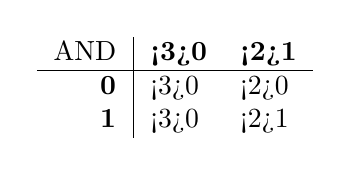
\begin{tikzpicture}
\node (and) {
\begin{tabular}{r|ll}
    AND & \bf \myemph<3>{0} & \bf \myemph<2>{1} \\ \hline
    \bf0 & \myemph<3>{0} & \myemph<2>{0} \\
    \bf1 & \myemph<3>{0} & \myemph<2>{1} \\
\end{tabular}
};
\end{tikzpicture}
    \begin{itemize}
        \item<2-> \myemph<2>{AND with 1}: keep a bit the same
        \item<3-> \myemph<3>{AND with 0}: clear a bit
        \vspace{.5cm}
        \item<4-> method: construct ``mask'' of what to keep/remove
    \end{itemize}
\end{frame}

\begin{frame}[fragile,label=bitwiseAnd]{bitwise AND --- {\tt \&}}
\begin{columns}[b]
\begin{column}{0.6\textwidth}
\lstset{
    moredelim=**[is][\btHL<1>]{@1*}{*@},
    moredelim=**[is][\btHL<2>]{@2*}{*@},
    moredelim=**[is][\btHL<3>]{@3*}{*@},
    moredelim=**[is][\btHL<4>]{@4*}{*@},
    moredelim=**[is][\btHL<5>]{@5*}{*@},
    moredelim=**[is][\btHL<6>]{@6*}{*@},
    escapechar=$,
}
\begin{itemize}
\item Treat value as \myemph{array of bits}
\item \lstinline|1 & 1 == 1|
\item \lstinline|1 & 0 == 0|
\item \lstinline|0 & 0 == 0|
\item \lstinline|@2*2 & 4 == 0*@|
\item \lstinline|@3*10 & 7 ==  2*@|
\end{itemize}
\vspace{0pt}
\end{column}
\begin{column}{0.4\textwidth}
\onslide<2->{
\tt
\begin{tabular}{llllll}
~  & \ldots & 0 & 0 & 1 & 0 \\
\&\hspace{.5cm} & \ldots & 0 & 1 & 0 & 0 \\\hline
~  & \ldots & 0 & 0 & 0 & 0
\end{tabular}
}
\vspace{1cm}
\onslide<3->{
\tt
\begin{tabular}{llllll}
~  & \ldots & 1 & 0 & 1 & 0 \\
\&\hspace{.5cm} & \ldots & 0 & 1 & 1 & 1 \\\hline
~  & \ldots & 0 & 0 & 1 & 0
\end{tabular}
}
\vspace{0pt}
\end{column}
\end{columns}
\end{frame}

\begin{frame}[fragile,label=bitwiseAndCAsm]{bitwise AND --- C/assembly}
    \begin{itemize}
    \item x86: {\tt {\keywordstyle and} \%reg, \%reg}
    \item C: \verb|foo & bar|
    \end{itemize}
\end{frame}

\begin{frame}[fragile,label=bitwiseHW]{bitwise hardware ({\tt10 \& 7 == 2})}
\begin{tikzpicture}[circuit logic US]
\node (num1) {\tt 10};
\coordinate (num1Intersect) at ($(num1) + (0, -1cm)$);
\draw[very thick] (num1) -- (num1Intersect);
\node[right=9cm of num1] (num2) {\tt 7};
\coordinate (num2Intersect) at ($(num2) + (0, -2cm)$);
\draw[very thick] (num2) -- (num2Intersect);

\matrix(ands) [
    below=2cm of num1,
    xshift=-.36cm,
    anchor=north west,
    matrix of nodes,
    column sep=.5cm,
    nodes={
        draw,
        fill=black!5,
        and gate,
        point down,
        logic gate inputs=nn
    }] {
    ~ \& |[draw=none,fill=none,rectangle]| \vdots \& ~ \& ~ \& ~ \& ~ \& ~ \& ~ \& ~ \\
};
\foreach \x in {1,3,4,5,6,7,8,9} {
    \draw[thin] ($(num1Intersect)-(0.4pt,0)+(0.\x pt,0)$) -- ($(num1Intersect) + (0mm,-2mm) + 3*(0.\x mm,0.\x mm)$) -| (ands-1-\x.input 2);
    \draw[thin] ($(num2Intersect)-(0.4pt,0)+(0.\x pt,0)$) -- ($(num2Intersect) + (0mm,-2mm) + 3*(-0.\x mm,0.\x mm)$) -| (ands-1-\x.input 1);
}
\begin{scope}[every node/.style={yshift=-1.2mm,font=\small\tt,xshift=1mm}]
\node[above left=0pt of ands-1-9.input 2] {0};
\node[above left=0pt of ands-1-8.input 2] {1};
\node[above left=0pt of ands-1-7.input 2] {0};
\node[above left=0pt of ands-1-6.input 2] {1};
\node[above right=0pt of ands-1-9.input 2] {1};
\node[above right=0pt of ands-1-8.input 2] {1};
\node[above right=0pt of ands-1-7.input 2] {1};
\node[above right=0pt of ands-1-6.input 2] {0};
\end{scope}
\begin{scope}[every node/.style={font=\small\tt}]
\node[below=1cm of ands-1-9.output] (res9) {0};
\node[below=1cm of ands-1-8.output] (res8) {1};
\node[below=1cm of ands-1-7.output] (res7) {0};
\node[below=1cm of ands-1-6.output] (res6) {0};
\end{scope}
\foreach \x in {1,3,4,5} {
    \coordinate (res\x) at ($(ands-1-\x.output) + (0,-1cm)$);
}
\foreach \x in {1,3,4,5,6,7,8,9} {
    \draw[thin] (ands-1-\x.output) -- (res\x);
}

\end{tikzpicture}
\end{frame}




\begin{frame}[fragile,label=extractOp3]{extract 0x3 from 0x1234}
\begin{ccodeNL}
unsigned get_second_nibble1(unsigned value) {
    return (value >> 4) & 0xF; // 0xF: 00001111
    // like (value / 16) % 16
}
\end{ccodeNL}
{\small\tt aaaabbbbccccdddd $\rightarrow$ aaaabbbbcccc $\rightarrow$ 00000000cccc}
\vspace{1.5cm}
\begin{ccodeNL}
unsigned get_second_nibble2(unsigned value) {
    return (value & 0xF0) >> 4; // 0xF0: 11110000
         //    "mask and shift"
    // like (value % 256) / 16; 
}
\end{ccodeNL}
{\small\tt aaaabbbbccccdddd $\rightarrow$ 000000000cccc0000 $\rightarrow$ 00000000cccc}
\end{frame}

\begin{frame}[fragile,label=extractOp4]{extract 0x3 from 0x1234}
\begin{asmcodeNL}
get_second_nibble1_bitwise:
    movl %edi, %eax
    shrl $4, %eax
    andl $0xF, %eax
    ret

get_second_nibble2_bitwise:
    movl %edi, %eax
    andl $0xF0, %eax
    shrl $4, %eax
    ret
\end{asmcodeNL}
\end{frame}


\subsection{or/xor}

\usetikzlibrary{arrows.meta,calc,positioning,decorations.pathreplacing}

\begin{frame}[fragile,label=bitwiseReasons]{and/or/xor}
\begin{tikzpicture}
\node (and) {
\color{red!50!black}
\begin{tabular}{r|ll}
AND & \bf 0 & \bf 1 \\ \hline
\bf0 & 0 & 0 \\
\bf1 & 0 & 1 \\
\end{tabular}
};
\node[right=2.5cm of and] (or) {
\color{blue!50!black}
\begin{tabular}{r|ll}
OR & \bf0 & \bf1 \\ \hline
\bf0 & 0 & 1 \\
\bf1 & 1 & 1 \\
\end{tabular}
};
\node[right=2.5cm of or] (xor) {
\color{green!50!black}
\begin{tabular}{r|ll}
XOR & \bf0 & \bf1 \\ \hline
\bf0 & 0 & 1 \\
\bf1 & 1 & 0 \\
\end{tabular}
};
\node[below=.5cm of and] {
    \color{red!50!black}\lstinline|&|
};
\node[below=1.5cm of and,align=left] (and why) {
    \color{red!50!black}conditionally clear bit \\
    \color{red!50!black}conditionally keep bit
};
\node[below=.5cm of and why, align=left,font=\fontsize{9}{10}\selectfont] {
    mask: 0s = clear; 1s = keep \\
    e.g. 101010101\ldots = \\ clear every other bit
};
\node[below=.5cm of or] {
    \color{blue!50!black}\lstinline+|+
};
\node[below=1.5cm of or] (or why) {
    \color{blue!50!black}conditionally set bit \\
};
\node[below=1.5cm of or why, align=left,font=\fontsize{9}{10}\selectfont] {
    mask: 1s = set; 0s = keep same \\
    e.g. 101010101\ldots = \\ set every other bit
};
\node[below=.5cm of xor] {
    \color{green!50!black}\lstinline+^+
};
\node[below=1.5cm of xor]  (xor why) {
    \color{green!50!black}conditionally flip bit
};
\node[below=1.5cm of xor why, align=left,font=\fontsize{9}{10}\selectfont] {
    mask: 1s = flip; 0s = keep same \\
};
\end{tikzpicture}
\end{frame}


\usetikzlibrary{arrows.meta,calc,positioning,decorations.pathreplacing}

\begin{frame}<2>[fragile,label=bitwiseOr]{bitwise OR --- {\tt |}}
\begin{columns}[b]
\begin{column}{0.6\textwidth}
\lstset{
    moredelim=**[is][\btHL<1>]{@1*}{*@},
    moredelim=**[is][\btHL<2|handout:0>]{@2*}{*@},
    moredelim=**[is][\btHL<3|handout:0>]{@3*}{*@},
    moredelim=**[is][\btHL<4>]{@4*}{*@},
    moredelim=**[is][\btHL<5>]{@5*}{*@},
    moredelim=**[is][\btHL<6>]{@6*}{*@},
    escapechar=$,
}
\begin{itemize}
\item \lstinline!1 | 1 == 1!
\item \lstinline!1 | 0 == 1!
\item \lstinline!0 | 0 == 0!
\item \lstinline!2 | 4 == 6!
\item \lstinline!@2*10 | 7 ==  15*@!
\end{itemize}
\end{column}
\begin{column}{0.4\textwidth}
\onslide<2->{
\tt
\begin{tabular}{llllll}
~  & \ldots & 1 & 0 & 1 & 0 \\
|\hspace{.5cm} & \ldots & 0 & 1 & 1 & 1 \\\hline
~  & \ldots & 1 & 1 & 1 & 1
\end{tabular}
}
\vspace{0pt}
\end{column}
\end{columns}
\end{frame}

\begin{frame}<2>[fragile,label=bitwiseXor]{bitwise xor --- {\tt \^~}}
\begin{columns}[b]
\begin{column}{0.6\textwidth}
\lstset{
    moredelim=**[is][\btHL<1>]{@1*}{*@},
    moredelim=**[is][\btHL<2|handout:0>]{@2*}{*@},
    moredelim=**[is][\btHL<3|handout:0>]{@3*}{*@},
    moredelim=**[is][\btHL<4>]{@4*}{*@},
    moredelim=**[is][\btHL<5>]{@5*}{*@},
    moredelim=**[is][\btHL<6>]{@6*}{*@},
    escapechar=$,
}
\begin{itemize}
\item \lstinline!1 ^ 1 == 0!
\item \lstinline!1 ^ 0 == 1!
\item \lstinline!0 ^ 0 == 0!
\item \lstinline!2 ^ 4 == 6!
\item \lstinline!@2*10 ^ 7 ==  13*@!
\end{itemize}
\end{column}
\begin{column}{0.4\textwidth}
\onslide<2->{
\tt
\begin{tabular}{llllll}
~  & \ldots & 1 & 0 & 1 & 0 \\
\lstinline|^|\hspace{.5cm} & \ldots & 0 & 1 & 1 & 1 \\\hline
~  & \ldots & 1 & 1 & 0 & 1
\end{tabular}
}
\vspace{0pt}
\end{column}
\end{columns}
\end{frame}

\begin{frame}[fragile,label=negation]{negation / not --- {\tt\textasciitilde}}
\lstset{
    moredelim=**[is][\btHL<1>]{@1*}{*@},
    moredelim=**[is][\btHL<2>]{@2*}{*@},
    moredelim=**[is][\btHL<3>]{@3*}{*@},
    moredelim=**[is][\btHL<4>]{@4*}{*@},
    moredelim=**[is][\btHL<5>]{@5*}{*@},
    moredelim=**[is][\btHL<6>]{@6*}{*@},
    moredelim=**[is][\it]{@*}{*@},
    escapechar=$,
}
\lstinline|~| (`complement') is bitwise version of \lstinline|!|:
\begin{columns}[t]
\begin{column}{0.6\textwidth}
\begin{itemize}
\item \lstinline|!0 == 1|
\item \lstinline|!notZero == 0|
\item \lstinline|~0 == (int) 0xFFFFFFFF| {\small (aka \lstinline|-1|)}
\item<2-> \lstinline|~2 == (int) 0xFFFFFFFD| {\small (aka \lstinline|-3|)}
\item<3-> \lstinline|~((unsigned) 2) == 0xFFFFFFFD|
\end{itemize}

\vspace{0pt}
\end{column}
\begin{column}{0.4\textwidth}
\vspace{2cm}

\tt
\begin{tabular}{llllllll}
\lstinline|~| \hspace{.5cm}& \tikzmark{s}0 & 0 & \ldots & 0 & 0 & 0 & 0\tikzmark{e} \\ \hline
 ~ & 1 & 1 & \ldots & 1 & 1 & 1 & 1 \\
\end{tabular}
\vspace{0pt}
\end{column}
\end{columns}
\begin{tikzpicture}[remember picture,overlay]
    \draw[decorate,thick,decoration={brace,amplitude=10pt}] ([yshift=1.5ex]pic cs:s) -- ([yshift=1.5ex]pic cs:e) node[midway,yshift=4ex] {32 bits};
\end{tikzpicture}
\end{frame}



\section{bit puzzles}

\begin{frame}{bit-puzzles}
\begin{itemize}
    \item assignments: bit manipulation puzzles
    \vspace{.5cm}
    \item solve some problem with bitwise ops
        \begin{itemize}
        \item maybe that you could do with normal arithmetic, comparisons, etc.
        \end{itemize}
    \item why?
        \begin{itemize}
        \item good for thinking about HW design
        \item good for understanding bitwise ops
        \item unreasonably common interview question type
        \end{itemize}
    \end{itemize}
\end{frame}


\subsection{case study: ternary operator}
% FIXME: try to simplify?
\begin{frame}[fragile,label=ternaryOp]{note: ternary operator}
    \begin{itemize}
    \item \lstinline|w = (x ? y : z)|
    \item \lstinline|if (x) { w = y; } else { w = z; }|
    \end{itemize}
\end{frame}


\subsubsection{options to simplify}
\begin{frame}[fragile,label=ternarySimplifyOptions]{ternary as bitwise: simplifying}
    \begin{itemize}
    \item \lstinline|(x ? y : z)| {\small \lstinline|if (x) return y; else return z;|}
    \item task: turn into non-if/else/etc. operators
        \begin{itemize}
        \item assembly: no jumps probably
        \end{itemize}
    \vspace{.5cm}
    \item strategy today: build a solution from simpler subproblems
        \begin{itemize}
        \item (1) with x, y, z 1 bit: \lstinline|(x ? y : 0)| and \lstinline|(x ? 0 : z)|
        \item (2) with x, y, z 1 bit: \lstinline|(x ? y : z)|
        \item (3) with x 1 bit: \lstinline|(x ? y : z)|
        \item (4) \lstinline|(x ? y : z)|
        \end{itemize}
    \end{itemize}
\end{frame}


\subsubsection{one-bit case}
\begin{frame}[fragile,label=exTernaryOneBit]{one-bit ternary}
\begin{itemize}
    \item \lstinline|(x ? y : z)|
    \item constraint: \textit{x, y, and z are 0 or 1}
    \item now: reimplement in C without if/else/\lstinline+||+/etc.
        \begin{itemize}
        \item (assembly: no jumps probably)
        \end{itemize}
    \vspace{.5cm}
    \item<2> divide-and-conquer:
        \begin{itemize}
            \item \lstinline|(x ? y : 0)|
            \item \lstinline|(x ? 0 : z)|
        \end{itemize}
\end{itemize}
\end{frame}

\begin{frame}[fragile,label=exTernaryOneBitParts]{one-bit ternary parts (1)}
\begin{itemize}
    \item constraint: \textit{x, y, and z are 0 or 1}
    \vspace{.5cm}
\item \lstinline|(x ? y : 0)| 
    \vspace{.5cm}
\item<2->
\begin{tabular}{r|ll}
    ~ & \bf y=0 & \bf y=1 \\ \hline
    \bf x=0 & 0 & 0 \\
    \bf x=1 & 0 & 1 \\
\end{tabular}
\item<2-> $\rightarrow$ \lstinline|(x & y)|
\end{itemize}
\end{frame}

\begin{frame}[fragile,label=exTernaryOneBitParts2]{one-bit ternary parts (2)}
\begin{itemize}
\item \lstinline|(x ? y : 0)| = \lstinline|(x & y)|
    \vspace{.5cm}
\item<2-> \lstinline|(x ? 0 : z)|
\item<2-> opposite \lstinline|x|: \lstinline|~x|
\item<2-> \lstinline|((~x) & z)|
\end{itemize}
\end{frame}

\begin{frame}[fragile,label=exTernaryOneBitCombine]{one-bit ternary}
    \begin{itemize}
        \item constraint: \textit{x, y, and z are 0 or 1}
        \item \lstinline|(x ? y : z)|
        \item {\color{green!70!black}\lstinline+(x ? y : 0)+}\lstinline+ | +{\color{blue!70!black}\lstinline+(x ? 0 : z)+}
        \item {\color{green!70!black}\lstinline+(x & y)+}\lstinline+ | +{\color{blue!70!black}\lstinline+((~x) & z)+}
    \end{itemize}
\end{frame}


\subsubsection{multi-bit x/y}
\begin{frame}<1-2>[fragile,label=exTernaryMultiProblem]{multibit ternary}
    \begin{itemize}
        \item constraint: \lstinline|x| \textit{is 0 or 1}
        \item old solution \lstinline+((x & y) | (~x) & z) + only gets least sig. bit
        \item \lstinline|(x ? y : z)|
        \item<2-> {\color{green!70!black}\lstinline+(x ? y : 0)+}\lstinline+ | +{\color{blue!70!black}\lstinline+(x ? 0 : z)+}
        \item<3-> {\color{green!70!black}\lstinline+((-x) & y)+}\lstinline+ | +{\color{blue!70!black}\lstinline+((-(x ^ 1)) & z)+}
    \end{itemize}
\end{frame}

\begin{frame}<1-2>[fragile,label=exTernaryMulti1]{constructing masks}
    \begin{itemize}
        \item constraint: \lstinline|x| \textit{is 0 or 1}
        \item \lstinline|(x ? y : 0)|
        \item turn into \lstinline|y & MASK|, where MASK = ???
            \begin{itemize}
            \item ``keep certain bits''
            \end{itemize}
        \item<2-> if x = 1: want {\tt 1111111111\ldots1} (keep {\tt y})
        \item<2-> if x = 0: want {\tt 0000000000\ldots0} (want {\tt 0})
            \vspace{.5cm}
        \item<3-> a trick: \lstinline|-x| ({\tt -1} is {\tt 1111\ldots1})
        \item<4-> \lstinline[basicstyle=\color{red}\tt]|((-x) & y)|
    \end{itemize}
\end{frame}

\againframe<3>{exTernaryMulti1}

% FIXME: example with numbers?

\begin{frame}[fragile,label=exTernaryMulti2]{constructing other masks}
    \begin{itemize}
        \item constraint: \lstinline|x| \textit{is 0 or 1}
        \item \lstinline|(x ? 0 : z)|
        \item if x = \xcancel{1} 0: want {\tt 1111111111\ldots1}
        \item if x = \xcancel{0} 1: want {\tt 0000000000\ldots0}
        \item mask: \xcancel{\tt -x} \begin{visibleenv}<2-> \lstinline|-(x^1)|\end{visibleenv}
    \end{itemize}
\end{frame}

\againframe<3>{exTernaryMultiProblem}


\subsubsection{multi-bit everything}
\begin{frame}<1-3>[fragile,label=exTernaryMultiFull]{fully multibit}
    \begin{itemize}
        \item ~$\xcancel{\text{constraint: {\tt x} is 0 or 1}}$
        \item \lstinline|(x ? y : z)|
        \item<2-> easy C way: {\tt !x} = 1 (if $x=0$) or 0, {\tt !(!x)} = 0 or 1
            \begin{itemize}
            \item x86 assembly: {\tt testq \%rax, \%rax} then {\tt sete/setne}
            \item (copy from ZF)
            \end{itemize}
        \item<3-> {\color{green!70!black}\lstinline+(x ? y : 0)+}\lstinline+ | +{\color{blue!70!black}\lstinline+(x ? 0 : z)+}
        \item<3-> {\color{green!70!black}\lstinline+((-!!x) & y)+}\lstinline+ | +{\color{blue!70!black}\lstinline+((-!x) & z)+}
    \end{itemize}
\end{frame}



% FIXME: skip?
\begin{frame}{simple operation performance}
    \begin{itemize}
    \item typical modern desktop processor:
        \begin{itemize}
        \item bitwise and/or/xor, shift, add, subtract, compare --- $\sim$ 1 cycle
        \item integer multiply --- $\sim$ 1-3 cycles
        \item integer divide --- $\sim$ 10-150 cycles
        \end{itemize}
    \item (smaller/simpler/lower-power processors are different)
    \vspace{.5cm}
    \item<2-> add/subtract/compare are more complicated in hardware!
    \item<2-> but \textit{much} more important for \myemph{typical applications}
    \end{itemize}
\end{frame}

\subsection{case study: any-bit?}

\usetikzlibrary{arrows.meta,calc,circuits.logic.US,fit,matrix,positioning}

\subsubsection{problem setup}


\begin{frame}[fragile,label=anyBit]{problem: any-bit}
    \begin{itemize}
        \item is any bit of {\tt x} set?
    \item goal: turn 0 into 0, not zero into 1
    \item easy C solution: \lstinline|!(!(x))|
        \begin{itemize}
        \item another solution if you have \lstinline|-| or \lstinline|+| (\texttt{bang} in lab)
        \end{itemize}
    \item what if we don't have \lstinline|!| or \lstinline|-| or \lstinline|+|
        \begin{itemize}
        \item more like what real hardware components to work with are
        \end{itemize}
    \vspace{.5cm}
    \item<2-> how do we solve is {\tt x} is, say, four bits?
    \item<3-> {\small\lstinline+((x & 1) | ((x >> 1) & 1) | ((x >> 2) & 1) | ((x >> 3) & 1))+}
    \end{itemize}
\end{frame}

\subsubsection{wasted work with naive 4 bit soln}

\begin{frame}[fragile,label=wastedAnyBitAnd]{wasted work (1)}
    \begin{itemize}
    \item {\small\lstinline+((x & 1) | ((x >> 1) & 1) | ((x >> 2) & 1) | ((x >> 3) & 1))+}
    \item in general: \lstinline+(x & 1) | (y & 1) == (x | y) & 1+
        \begin{itemize}
        \item distributive property
        \end{itemize}
        \vspace{.5cm}
    \item<2-> {\small\lstinline+(x | (x >> 1) | (x >> 2) | (x >> 3)) & 1+}
    \end{itemize}
\end{frame}

\begin{frame}[fragile,label=wastedAnyBitOrs]{wasted work (2)}
    \lstset{
        language=C,
        moredelim=**[is][\btHL<1>]{@1}{1@}
    }
    \begin{itemize}
    \item 4-bit any set: {\small\lstinline+(@1x | (x >> 1)1@ | (x >> 2) | (x >> 3)) & 1+}
    \item performing 3 bitwise ors
    \item \ldots each bitwise or does 4 OR operations
    \item<2> but only result of one of the 4!
    \end{itemize}
\begin{tikzpicture}[circuit logic US]
\coordinate (num1Intersect) at (0, 0);
\coordinate (num2Intersect) at (0, -0.5);
    \matrix(ors) at (0, -1)[
    xshift=-.36cm,
    anchor=north west,
    matrix of nodes,
    column sep=.5cm,
    nodes={
        draw,
        fill=black!5,
        or gate,
        point down,
        logic gate inputs=nn
    }] {
    ~ \& ~ \& ~ \& ~  \\
};
\foreach \x in {1,2,3,4} {
    \draw[thin] ($(num1Intersect)-(0.4pt,0)+(0.\x pt,0)$) -- ($(num1Intersect) + (0mm,-2mm) + 3*(0.\x mm,0.\x mm)$) -| (ors-1-\x.input 2);
    \draw[thin] ($(num2Intersect)-(0.4pt,0)+(0.\x pt,0)$) -- ($(num2Intersect) + (0mm,-2mm) + 3*(-0.\x mm,0.\x mm)$) -| (ors-1-\x.input 1);
}
    \node [left=0cm of num1Intersect] { \lstinline|(x)| };
    \node [left=0cm of num2Intersect] { \lstinline|(x >> 1)| };
    \node[draw,red,very thick,fit=(ors-1-4)] {};
\end{tikzpicture}
\end{frame}


\begin{frame}[fragile,label=divideAndCongMotiv]{any-bit: looking at wasted work}
\begin{tikzpicture}
\tikzset{
    >=Latex,
    hidden zero/.style={black!70},
    hidden wrong col/.style={black!40},
    hilite used/.style={fill=red!20},
}
\matrix[
    tight matrix,
    nodes={draw=none,text width=2.5cm,align=center},
    anchor=north east,
    alt=<1>{row 3/.style={nodes={invisible}}}
] (fan in)  {
    $x_3$ \& $x_2$ \& $x_1$ \& $x_0$ \\[.5cm]
    |[hidden zero]| $0$   \& $x_3$ \& $x_2$ \& $x_1$ \\[1.5cm]
    $(0|x_3)$ \& |[hilite used]| $(x_3|x_2)$ \& $(x_2|x_1)$ \& |[hilite used]| $(x_1|x_0)$ \\[.5cm]
};
    \foreach \r/\s in {1/x,2/x>>1,3/y=(x|x>>1)} {
        \node[anchor=west] at ([xshift=0.25cm]fan in-\r-4.east) {\tt \s};
    }
    \foreach \tFrom/\tTo in {1/2,2/3,3/4} {
        \draw[very thick,->] (fan in-1-\tFrom) -- (fan in-2-\tTo);
    }
    \begin{visibleenv}<3>
        \node[draw=red,very thick,anchor=north,align=left] at (fan in.south) {
            final value wanted: $x_3|x_2|x_1|x_0$  \\
            previously: \\
            \hspace{2cm} compute {\tt x|(x>>1)} for $x_1|x_0$; \\
            \hspace{2cm} {\tt (x>>2)|(x>>3)} for $x_3|x_2$ \\
            observation: got both parts with just {\tt x|(x>>1)}
        };
    \end{visibleenv}
\end{tikzpicture}
\end{frame}

\subsubsection{a divide and conquer solution}

\begin{frame}[fragile,label=divideAndConq2]{any-bit: divide and conquer}
\begin{tikzpicture}
\tikzset{
    >=Latex,
    hidden zero/.style={black!70},
    hidden wrong col/.style={black!40},
}
\matrix[
    tight matrix,
    nodes={draw=none,text width=2.5cm,align=center},
    anchor=north east,
] (fan in)  {
    $x_3$ \& $x_2$ \& $x_1$ \& $x_0$ \\[.5cm]
    |[hidden zero]| $0$   \& $x_3$ \& $x_2$ \& $x_1$ \\[1.5cm]
    |[hidden wrong col]| $(0|x_3)$ \& $(x_3|x_2)$ \& |[hidden wrong col]| $(x_2|x_1)$ \& $(x_1|x_0)$ \\[.5cm]
    |[hidden wrong col]| $0$ \& |[hidden zero]| $0$ \& |[hidden wrong col]| $(0|x_3)$ \& $(x_3|x_2)$ \\[1.5cm]
    |[hidden wrong col]| $x_3$ \& |[hidden wrong col]| $(x_3|x_2)$\& |[hidden wrong col]| $(x_3|x_2|x_1)$ \& $(x_3|x_2|x_1|x_0)$ \\
};
    \foreach \r/\s in {1/x,2/x>>1,3/y=(x>>1)|x,4/y>>2,5/y|(y>>2)} {
        \node[anchor=west] at ([xshift=0.25cm]fan in-\r-4.east) {\tt \s};
    }
    \foreach \tFrom/\tTo in {1/2,3/4} {
        \draw[very thick,->] (fan in-1-\tFrom) -- (fan in-2-\tTo);
    }
    \foreach \tFrom/\tTo in {2/2,4/4} {
        \draw[very thick,->] (fan in-2-\tFrom) -- (fan in-3-\tTo);
    }
    \foreach \tFrom/\tTo in {2/4} {
        \draw[very thick,->] (fan in-3-\tFrom) -- (fan in-4-\tTo);
    }
    \foreach \tFrom/\tTo in {4/4} {
        \draw[very thick,->] (fan in-4-\tFrom) -- (fan in-5-\tTo);
    }
\end{tikzpicture}
\end{frame}

\begin{frame}[fragile,label=divideConquery]{any-bit: divide and conquer}
    \begin{itemize}
    \item ~
    \item ~
    \item four-bit input $x=x_3x_2x_1x_0$
    \item \lstinline+x | (x >> 1)+ = $(x_3|0)\myemph{(x_2|x_3)}(x_1|x_2)\myemph{(x_0|x_1)}=y_1\myemph{y_2}y_3\myemph{y_4}$
    \item<2-> \lstinline+y | (y >> 2)+ = $(y_1|0)(y_2|0)(y_3|y_1)\myemph{(y_4|y_2)}=z_1z_2z_3z_4$
    \item<2-> $z_4=(y_4|y_2)=((x_2|x_3)|(x_0|x_1))=x_0|x_1|x_2|x_3$ ``is any bit set?''
\begin{visibleenv}<3->
    \vspace{.5cm}
\begin{ccodeNL}
unsigned int any_of_four(unsigned int x) {
    int part_bits = (x >> 1) | x;
    return ((part_bits >> 2) | part_bits) & 1;
}
\end{ccodeNL}
\end{visibleenv}
    \end{itemize}
\begin{tikzpicture}[overlay,remember picture]
\tikzset{>=Latex}
\coordinate (fan top left) at ([xshift=-2cm,yshift=-1cm]current page.north east);
\matrix[
    tight matrix,
    nodes={draw=none,text width=1.5cm,align=center},
    anchor=north east,
    row sep=5mm,
] (fan in) at (fan top left) {
    $x_3$ \& $x_2$ \& $x_1$ \& $x_0$ \\
    ~\& $(x_3|x_2)$ \& ~ \& $(x_1|x_0)$ \\\
    ~\& ~\&~ \& $(x_3|x_2|x_1|x_0)$\\
};
    \foreach \tFrom/\tTo in {1/2,2/2,3/4,4/4} {
        \draw[very thick,->] (fan in-1-\tFrom.south) -- (fan in-2-\tTo.north);
    }
    \foreach \tFrom/\tTo in {2/4,4/4} {
        \draw[very thick,->] (fan in-2-\tFrom.south) -- (fan in-3-\tTo.north);
    }
\end{tikzpicture}
\end{frame}

\begin{frame}[fragile,label=divideAndConq8bit]{any-bit: divide and conquer}
\begin{tikzpicture}
\tikzset{
    >=Latex,
    hidden zero/.style={black!70},
    hidden wrong col/.style={black!40},
}
\matrix[
    tight matrix,
    nodes={draw=none,text width=1.5cm,font=\small,align=center},
    row 6/.style={nodes={font=\everymath{\scriptstyle}}},
    row 7/.style={nodes={font=\everymath{\scriptstyle}}},
    row 5/.style={nodes={font=\everymath{\scriptstyle}}},
    anchor=north east,
] (fan in)  {
    $x_7$ \& $x_6$ \& $x_5$ \& $x_4$ \& $x_3$ \& $x_2$ \& $x_1$ \& $x_0$ \\[.5cm]
    |[hidden zero]| $0$  \& $x_7$ \& $x_6$ \& $x_5$ \& $x_4$ \& $x_3$ \& $x_2$ \& $x_1$ \\[1.5cm]
    |[hidden wrong col]| $(0|x_7)$ \& $(x_7|x_6)$ \& |[hidden wrong col]| $(x_6|x_5)$ \& $(x_5|x_4)$ \& |[hidden wrong col]|  $(x_4|x_3)$ \& $(x_3|x_2)$ \& |[hidden wrong col]| $(x_2|x_1)$ \& $(x_1|x_0)$ \\[.5cm]
    |[hidden wrong col]| $0$ \& |[hidden wrong col]| $0$ \& 
    |[hidden wrong col]| $(0|x_7)$ \& $(x_7|x_6)$ \& 
    |[hidden wrong col]| $(x_6|x_5)$ \& 
    |[hidden wrong col]| $(x_5|x_4)$ \& |[hidden wrong col]| $(x_4|x_3)$ \& $(x_3|x_2)$ \\[1.5cm]
    |[hidden wrong col]| $(0|0|0|x_7)$ \& ~ \&
    |[hidden wrong col]| $(0|x_7|x_6|x_5)$ \& ~ \&
    |[hidden wrong col]| $(x_6|x_5|x_4|x_3)$ \& ~ \&
    |[hidden wrong col]| $(x_4|x_3|x_2|x_1)$ \& ~ \\[-0cm]
    ~ \& |[hidden wrong col]| $(0|0|x_7|x_6)$ \& 
    ~ \& $(x_7|x_6|x_5|x_4)$ \& 
    ~ \& |[hidden wrong col]| $(x_5|x_4|x_3|x_2)$ \&
    ~ \& $(x_3|x_2|x_1|x_0)$ \\[.5cm]
};
    \foreach \r/\s in {1/x,2/x>>1,3/y=(x>>1)|x,4/y>>2,5/z=y|(y>>2)} {
        \node[anchor=west,font=\small] at ([xshift=0.25cm]fan in-\r-8.east) {\tt \s};
    }
    \foreach \tFrom/\tTo in {1/2,3/4,5/6,7/8} {
        \draw[very thick,->] (fan in-1-\tFrom) -- (fan in-2-\tTo);
    }
    \foreach \tFrom/\tTo in {2/2,4/4,6/6,8/8} {
        \draw[very thick,->] (fan in-2-\tFrom) -- (fan in-3-\tTo);
    }
    \foreach \tFrom/\tTo in {1/1,3/3,5/5,7/7} {
        \draw[thick,->,hidden wrong col,dotted] (fan in-2-\tFrom) -- (fan in-3-\tTo);
    }
    \foreach \tFrom/\tTo in {2/4,6/8} {
        \draw[very thick,->] (fan in-3-\tFrom) -- (fan in-4-\tTo);
    }
    \foreach \tFrom/\tTo in {4/4,8/8} {
        \draw[very thick,->] (fan in-4-\tFrom) -- (fan in-5-\tTo);
    }
\end{tikzpicture}
\end{frame}


\begin{frame}[fragile,label=anyBitSolution]{any-bit-set: 32 bits}
\begin{ccodeNL}
unsigned int any(unsigned int x) {
    x = (x >> 1) | x;
    x = (x >> 2) | x;
    x = (x >> 4) | x;
    x = (x >> 8) | x;
    x = (x >> 16) | x;
    return x & 1;
}
\end{ccodeNL}
\end{frame}



\subsection{general strategies}

\begin{frame}[fragile,label=bitStrat]{bitwise strategies}
    \begin{itemize}
        \item use paper, find subproblems, etc.
        \item mask and shift 
            \begin{itemize}
                \item \lstinline+(x & 0xF0) >> 4+
            \end{itemize}
        \item factor/distribute
            \begin{itemize}
                \item \lstinline+(x & 1) | (y & 1) == (x | y) & 1+
            \end{itemize}
        \item divide and conquer
        \item common subexpression elimination
            \begin{itemize}
                \item \lstinline+return ((-!!x) & y) | ((-!x) & z)+
                \item becomes
                \item \lstinline+d = !x; return ((-!d) & y) | ((-d) & z)+
            \end{itemize}
    \end{itemize}
\end{frame}




\section{bitwise exercise}
\begin{frame}[fragile,label=exercise]{exercise}
\begin{itemize}
    \item Which of these will swap least significant and second least significant bit of an {\tt unsigned int} $x$?    
        (bits $uvwxyz$ become $uvwxzy$)
\end{itemize}
\begin{ccodeS*}{texcomments=false}
/* version A */ 
    return ((x >> 1) & 1) | (x & (~1));

/* version B */
    return ((x >> 1) & 1) | ((x << 1) & (~2)) | (x & (~3));

/* version C */
    return (x & (~3)) | ((x & 1) << 1) | ((x >> 1) & 1);

/* version D */
    return (((x & 1) << 1) | ((x & 3) >> 1)) ^ x;

\end{ccodeS*}
\end{frame}

\begin{frame}[fragile,label=exerciseA]{version A}
\begin{ccodeS*}{texcomments=false}
/* version A */ 
    return ((x >> 1) & 1) | (x & (~1));
    //     ^^^^^^^^^^^^^^
    //      uvwxyz --> 0uvwxy -> 00000y

    //                      ^^^^^^^^^^
    //      uvwxyz --> uvwxy0

    //     ^^^^^^^^^^^^^^^^^^^^^^^^^^^ 
    //      00000y | uvwxy0 = uvwxyy 
\end{ccodeS*}
\end{frame}

\begin{frame}[fragile,label=exerciseB]{version B}
\begin{ccodeS*}{texcomments=false}
/* version B */
    return ((x >> 1) & 1) | ((x << 1) & (~2)) | (x & (~3));
    //     ^^^^^^^^^^^^^^
    //      uvwxyz --> 0uvwxy --> 00000y

    //                       ^^^^^^^^^^^^^^^
    //      uvwxyz --> vwxyz0 --> vwxy00

    //                                          ^^^^^^^^^ 
    //      uvwxyz -->            uvwx00
\end{ccodeS*}
\end{frame}

\begin{frame}[fragile,label=exerciseC]{version C}
\begin{ccodeS*}{texcomments=false}
/* version C */
    return (x & (~3)) | ((x & 1) << 1) | ((x >> 1) & 1);
    //     ^^^^^^^^^^
    //      uvwxyz -->            uvwx00

    //                  ^^^^^^^^^^^^^^
    //      uvwxyz --> 00000z --> 0000z0

    //                                   ^^^^^^^^^^^^^ 
    //      uvwxyz --> 0uvwxy --> 00000y
\end{ccodeS*}
\end{frame}

\begin{frame}[fragile,label=exerciseD]{version D}
\begin{ccodeS*}{texcomments=false}
/* version D */
    return (((x & 1) << 1) | ((x & 3) >> 1)) ^ x;
    //     ^^^^^^^^^^^^^^^
    //      uvwxyz --> 00000z --> 0000z0

    //                        ^^^^^^^^^^^^^^
    //      uvwxyz --> 0000yz --> 00000y

    //      ^^^^^^^^^^^^^^^^^^^^^^^^^^^^^^^^^^^^
    //      0000zy ^ uvwxyz --> uvwx(z XOR y)(y XOR z)
\end{ccodeS*}
\end{frame}

\begin{frame}[fragile,label=exResult]{expanded code}
\begin{ccodeS}
int lastBit = x & 1;
int secondToLastBit = x & 2;
int rest = x & ~3;
int lastBitInPlace = lastBit << 1;
int secondToLastBitInPlace = secondToLastBit >> 1;
return rest | lastBitInPlace | secondToLastBitInPlace;
\end{ccodeS}
\end{frame}


\section{backup slides}
\begin{frame}{backup slides}
\end{frame}


\subsection{misc. bitwise operations}
\begin{frame}{miscellaneous bit manipulation}
    \begin{itemize}
    \item common bit manipulation instructions are not in C:
    \vspace{.5cm}
    \item rotate (x86: {\tt ror}, {\tt rol}) --- like shift, but wrap around
    \item first/last bit set (x86: {\tt bsf}, {\tt bsr})
    \item population count (some x86: {\tt popcnt}) --- number of bits set
    \item byte swap: (x86: {\tt bswap})
    \end{itemize}
\end{frame}


\end{document}
